% !TeX program = xelatex
% AI 根据研究讨论生成的组内讨论草稿；使用 Codex 内置编译器。
% 本文件记录理论推导；实验汇总分别见 Experiment1、Experiment2、Experiment3。
% 当前范围：重整化与混合、双 coupling 算法、三网络高斯路径、Matching，以及与 WFR-FM 的关系。
% 排版约定：大节使用 \subsection*，节内推导步骤使用 \paragraph。
\documentclass[UTF8,a4paper,11pt,fontset=fandol]{ctexart}

\usepackage[margin=25mm]{geometry}
\usepackage{amsmath,amssymb,bm,mathrsfs}
\usepackage{graphicx}
\usepackage[unicode,hidelinks]{hyperref}

\pagestyle{plain}
\setcounter{secnumdepth}{0}
\ctexset{paragraph={format=\normalfont\normalsize\bfseries}}

\begin{document}

\begin{center}
{\LARGE\bfseries SimulationFree DeepRUOT\par}
\vspace{1.2em}
{\large\kaishu 环路总会有终点，谜题也总会有答案\par}
\end{center}
\vspace{0.6em}

\noindent\textbf{TL;DR：}
通过固定端点控制代价的重整化-路径混合手续，我们在不知道 DeepRUOT 对应的路径空间表述的情况下得到了控制代价的成对分解。
作为近似，删去这个代价中与后验生长、后验漂移有关的项，即得到可解的优化问题。
通过预先学习成对最优条件概率路径，再计算成对代价并求解 Coupling，最后对 Score, Drift, Growth 进行回归，
我们得到了一种 DeepRUOT 的近似的 Simulation Free 的求解方法。
实验结果表明，使用 WFR Coupling + WFR 均值 + WFR 质量 + 布朗桥方差即可实现对 DeepRUOT 问题最优控制律的较精确近似。

\vspace{1em}
\noindent\textbf{参考文献}
\begin{small}
\begin{itemize}
\setlength{\itemsep}{0.65em}
\setlength{\parsep}{0pt}
\item \textbf{DeepRUOT.}
Zhenyi Zhang, Tiejun Li, Peijie Zhou.
\emph{\href{https://openreview.net/forum?id=gQlxd3Mtru}{Learning Stochastic Dynamics from Snapshots through Regularized Unbalanced Optimal Transport}}.
ICLR, 2025.

\item \textbf{Variational RUOT.}
Yuhao Sun, Zhenyi Zhang, Zihan Wang, Tiejun Li, Peijie Zhou.
\emph{\href{https://arxiv.org/abs/2505.11823}{Variational Regularized Unbalanced Optimal Transport: Single Network, Least Action}}.
NeurIPS, 2025.

\item \textbf{WFR-FM.}
Qiangwei Peng, Zihan Wang, Junda Ying, Yuhao Sun, Qing Nie, Lei Zhang, Tiejun Li, Peijie Zhou.
\emph{\href{https://arxiv.org/abs/2601.06810}{WFR-FM: Simulation-Free Dynamic Unbalanced Optimal Transport}}.
ICLR, 2026.

\item \textbf{Beyond Continuity.}
Junda Ying, Yuxuan Wang, Bowen Yang, Peijie Zhou, Lei Zhang.
\emph{\href{https://arxiv.org/abs/2605.00545}{Beyond Continuity: Simulation-free Reconstruction of Discrete Branching Dynamics from Single-cell Snapshots}}.
arXiv:2605.00545, 2026.

\item \textbf{SUDO.}
Junda Ying, Yuxuan Wang, Bowen Yang, Peijie Zhou, Lei Zhang.
\emph{\href{https://arxiv.org/abs/2609.04710}{Simulation-free Unbalanced Dynamic Optimal Transport with General Growth Penalty}}.
arXiv:2609.04710, 2026.

\item \textbf{Score--Flow Matching.}
Alexander Y. Tong, Nikolay Malkin, Kilian Fatras, Lazar Atanackovic, Yanlei Zhang, Guillaume Huguet, Guy Wolf, Yoshua Bengio.
\emph{\href{https://proceedings.mlr.press/v238/tong24a.html}{Simulation-Free Schr\"odinger Bridges via Score and Flow Matching}}.
AISTATS, 2024.
\end{itemize}
\end{small}

\clearpage
\section*{实验结果}
在三个数据集上比较 RUOT 与 WFR 均值、质量曲线加布朗桥方差的基线
（图中记为 WFR+BB）。两者均取 $\alpha=10$、$\sigma=0.25$、$\psi(g)=g^2/2$。
使用训练好的反馈模型计算
\[
\operatorname{Action}
=\int\!\int\rho_t(x)\left(\frac12\|U_t(x)\|^2+\frac\alpha2G_t(x)^2\right)dx\,dt,
\qquad U=V+\frac{\sigma^2}{2}S.
\]
每个固定模型进行 20 次 Monte Carlo 评测，种子为 1000--1019；
同一数据集的两种方法在对应种子下共用初始抽样和布朗噪声。
每次使用 2000 个带权粒子，每单位时间积分 200 步。

\begin{figure}[!ht]
\centering
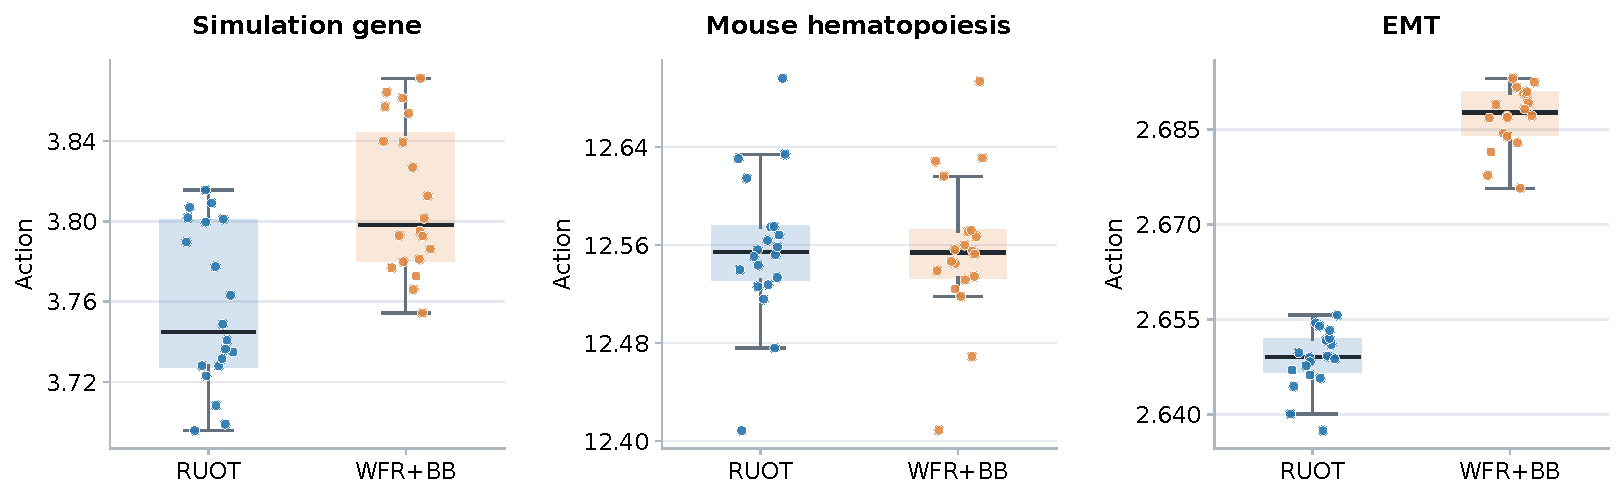
\includegraphics[width=\textwidth]{Experiment1/Figures/action_alpha10_three_datasets.pdf}
\caption{三个数据集上各 20 次 Action 评测的箱线图与全部散点。
箱体表示第一至第三四分位数，横线为中位数，须延伸至 $1.5$ 倍四分位距内的最远观测值；
散点的水平抖动仅用于显示。各面板分别使用纵轴尺度。
这些重复评测反映固定模型的推理 Monte Carlo 波动，不代表重复训练的波动。}
\label{fig:action-alpha10-three-datasets}
\end{figure}

\begin{figure}[!ht]
\centering
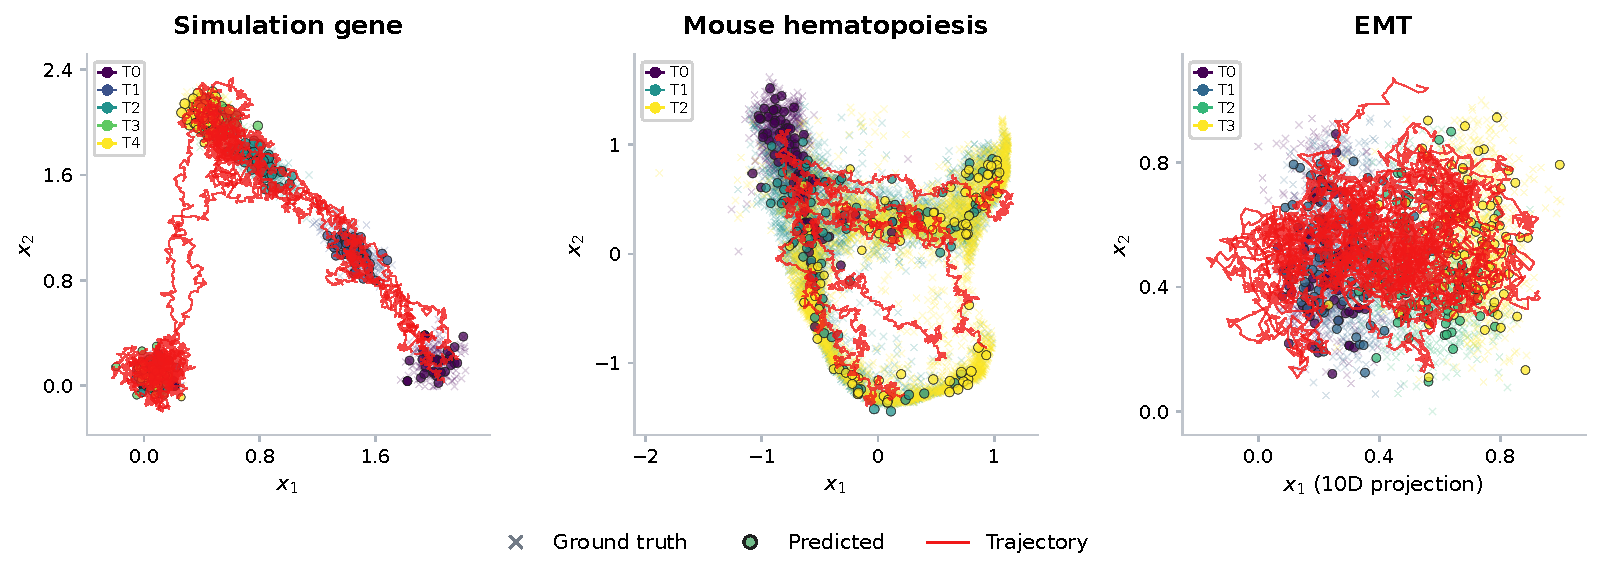
\includegraphics[width=\textwidth]{Experiment1/Figures/ruot_rollouts_three_datasets.pdf}
\caption{三个数据集的 RUOT 连续 rollout。颜色表示观测时间；叉号为真实样本，
圆点为每时刻随机展示的 80 个预测粒子，面积与粒子权重成正比；红线为随机选取的 8 条完整轨迹。
所有轨迹从初始时刻连续积分，中间不重启。EMT 展示完整十维演化的 $x_1/x_2$ 投影。}
\label{fig:ruot-rollout-three-datasets}
\end{figure}

\clearpage
\section*{正文}
\subsection*{成对粒子的重整化控制代价}
考虑时间区间 $[0,1]$ 上从 $(x_0,m_0)$ 到 $(x_1,m_1)$ 的带权条件路径，
其中 $x_0,x_1\in\mathbb R^d$、$m_0,m_1>0$。
用未归一化密度 $f_t(x)$ 描述该路径，记其总质量为
$m_t=\int_{\mathbb R^d}f_t(x)\,dx$。
漂移控制 $u_t(x)$ 和增长率 $g_t(x)$ 满足
\begin{equation}
\begin{aligned}
\partial_t f_t
&=-\nabla\cdot(f_tu_t)+\frac{\sigma^2}{2}\Delta f_t+g_tf_t,\\
f_0&=m_0\delta_{x_0},\qquad f_1=m_1\delta_{x_1},
\end{aligned}
\label{eq:pair-dynamics}
\end{equation}
其中扩散强度 $\sigma>0$、增长惩罚系数 $\alpha>0$ 为常数。
取任意给定的适当下半连续凸增长惩罚
$\psi:\mathbb R\to[0,+\infty]$；
$\psi(g)=g^2/2$ 对应此前的二次增长惩罚。
这里指定的初末质量是条件子群的总质量。
保留任意可行的控制 $(u,g)$，定义截断运行代价
\begin{equation}
C_\delta[f,u,g]
=\int_0^{1-\delta}\int_{\mathbb R^d}
f_t(x)\left(\frac12\|u_t(x)\|^2+\alpha\psi(g_t(x))\right)\,dx\,dt.
\label{eq:truncated-cost}
\end{equation}
在附录所列的布朗型末端渐近与可积性条件下，
其对数发散系数由末端质量 $m_1$ 决定：
\begin{equation}
C_\delta[f,u,g]
=\frac{d\sigma^2m_1}{2}\log\frac1\delta
+C_{\mathrm{ren}}[f,u,g]+o(1).
\label{eq:renormalization}
\end{equation}
引入辅助函数
\begin{equation}
v_t(x)=\frac{x_1-x}{1-t},
\qquad
F_t(x)=\frac{\|x-x_1\|^2}{2(1-t)},
\label{eq:comparison-fields}
\end{equation}
有限的重整化控制代价为
\begin{equation}
\boxed{
\begin{aligned}
C_{\mathrm{ren}}[f,u,g]
={}&\frac{m_0}{2}\|x_1-x_0\|^2-\frac{d\sigma^2m_1}{2}\\
&+\frac12\int_0^1\int_{\mathbb R^d}
f_t\|u_t-v_t\|^2\,dx\,dt\\
&+\int_0^1\int_{\mathbb R^d}
f_t\left(\alpha\psi(g_t)+g_tF_t\right)\,dx\,dt\\
&+\frac{d\sigma^2}{2}\int_0^1\frac{m_t-m_1}{1-t}\,dt.
\end{aligned}
}
\label{eq:renormalized-cost}
\end{equation}
式中 $v_t$ 仅作为平方配方的比较场；真实控制 $u_t,g_t$ 及密度路径 $f_t$
仍待优化。上式没有把整条条件路径预先指定为布朗桥或高斯路径，
其推导见附录。

\paragraph{直接优化成对路径.}
对给定的端点，将满足式 \eqref{eq:pair-dynamics}
及附录可积性条件的路径类记为 $\mathcal A$。成对最优代价定义为
\begin{equation}
c_{\mathrm{ren}}(x_0,m_0;x_1,m_1)
=\inf_{(f,u,g)\in\mathcal A}
C_{\mathrm{ren}}[f,u,g].
\label{eq:pair-optimization}
\end{equation}
我们可以直接最小化这个目标，无需先求解 HJB 方程。
若采用参数化路径，仍需保证密度、漂移与增长控制满足演化约束；
在受限路径族中优化时，得到的是该路径族内的近似解。

\clearpage
\subsection*{通过两个 coupling 混合终点并消去发散}

\paragraph{发射质量与接收质量.}
设初末质量密度为 $\mu_0,\mu_1$，其总质量可以不同。
用两张非负 coupling 密度分别描述每对端点的发射与接收质量：
\begin{equation}
\int_{\mathbb R^d}\pi^+(x_0,x_1)\,dx_1=\mu_0(x_0),
\qquad
\int_{\mathbb R^d}\pi^-(x_0,x_1)\,dx_0=\mu_1(x_1).
\label{eq:semicoupling-constraints}
\end{equation}
以下在 $\pi^+>0$ 且质量比有限、为正的配对上叙述。
记 $z=(x_0,x_1)$，并令
\begin{equation}
r_z=\frac{\pi^-(x_0,x_1)}{\pi^+(x_0,x_1)},
\qquad
q^+(x_1\mid x_0)=\frac{\pi^+(x_0,x_1)}{\mu_0(x_0)}.
\label{eq:pair-ratio}
\end{equation}
将每条条件路径按单位发射质量归一化，取
$f_0^z=\delta_{x_0}$、$f_1^z=r_z\delta_{x_1}$，
并保留对应的任意可行控制 $(u^z,g^z)$。
乘回 $\pi^+(z)$ 后，该分量的初末质量恰好分别为 $\pi^+(z)$ 和 $\pi^-(z)$。
记第一节给出的当前路径重整化代价为
$C_{\mathrm{ren}}^z=C_{\mathrm{ren}}[f^z,u^z,g^z]$。

\paragraph{固定起点后混合终点.}
先保留起点标签 $x_0$，对终点作混合：
\begin{equation}
p_t(x\mid x_0)
=\int_{\mathbb R^d}q^+(x_1\mid x_0)f_t^{x_0,x_1}(x)\,dx_1.
\label{eq:endpoint-mixture}
\end{equation}
$p_t$ 是每单位初始质量对应的质量密度，中间时刻的积分一般不等于 $1$。
在当前位置 $x$ 处，终点标签的质量后验为
\begin{equation}
\begin{aligned}
\omega_t(x_1\mid x,x_0)
&=\frac{q^+(x_1\mid x_0)f_t^{x_0,x_1}(x)}{p_t(x\mid x_0)}\\
&=\frac{\pi^+(x_0,x_1)f_t^{x_0,x_1}(x)}
{\int_{\mathbb R^d}\pi^+(x_0,y)f_t^{x_0,y}(x)\,dy}.
\end{aligned}
\label{eq:mass-posterior}
\end{equation}
用这个后验同时平均漂移和增长控制：
\begin{equation}
U_t^{x_0}(x)=\int\omega_t u_t^{x_0,x_1}(x)\,dx_1,
\qquad
G_t^{x_0}(x)=\int\omega_t g_t^{x_0,x_1}(x)\,dx_1.
\label{eq:mixed-controls}
\end{equation}
由通量和增长源的线性相加，混合密度满足
\begin{equation}
\begin{aligned}
\partial_t p_t
&=-\nabla\cdot(p_tU_t^{x_0})+\frac{\sigma^2}{2}\Delta p_t+G_t^{x_0}p_t,\\
p_0(x\mid x_0)&=\delta_{x_0}(x),
\qquad
p_1(x\mid x_0)=\frac{\pi^-(x_0,x)}{\mu_0(x_0)}.
\end{aligned}
\label{eq:mixed-dynamics}
\end{equation}
因此 $\int\mu_0(x_0)p_1(x\mid x_0)\,dx_0=\mu_1(x)$。
仅混合终点后的控制代价定义为
\begin{equation}
\mathcal T
=\int_0^1\int_{\mathbb R^d}\mu_0(x_0)
\int_{\mathbb R^d}p_t(x\mid x_0)
\left(\frac12\|U_t^{x_0}(x)\|^2+\alpha\psi(G_t^{x_0}(x))\right)
\,dx\,dx_0\,dt.
\label{eq:mixed-action}
\end{equation}
这里对起点质量的积分用于累计代价，控制本身仍保留起点标签。

\paragraph{有限的双 coupling 代价.}
为写出混合后的有限项，定义当前全体质量的积分记号
\begin{equation}
\langle A\rangle_t
:=\iint\pi^+(z)\int_{\mathbb R^d}f_t^z(x)A(t,z,x)\,dx\,dx_0\,dx_1.
\label{eq:mass-bracket}
\end{equation}
对于 $t>0$，定义漂移残差及其条件平均
\begin{equation}
\eta_t^z(x)
=u_t^z(x)-\frac{x-x_0}{t}-\sigma^2\nabla\log f_t^z(x),
\qquad
\bar\eta_t^{x_0}(x)=\int\omega_t\eta_t^z(x)\,dx_1.
\label{eq:drift-residual}
\end{equation}
这个分解不对 $u_t^z$ 增加约束；初端按极限处理。
混合修正由以下三个量给出：
\begin{equation}
\begin{aligned}
\widetilde{\mathcal K}_t
&=\langle g_t^z\log\omega_t\rangle_t,\\
\mathcal V_{\eta,t}
&=\langle\|\eta_t^z-\bar\eta_t^{x_0}\|^2\rangle_t,\\
\mathcal J_{\psi,t}
&=\langle\psi(g_t^z)-\psi(G_t^{x_0})\rangle_t\ge0.
\end{aligned}
\label{eq:mixture-corrections}
\end{equation}
最后一项是增长控制混合产生的 Jensen 差。
当 $\psi(g)=g^2/2$ 时，它等于
$\frac12\langle(g_t^z-G_t^{x_0})^2\rangle_t$；
一般凸惩罚下不把它写成方差。
在附录所列的连续终点、熵渐近和可积性条件下，
截断能量中的对数项恰好抵消，得到
\begin{equation}
\boxed{
\begin{aligned}
\mathcal T
={}&\iint\pi^+(z)C_{\mathrm{ren}}^z\,dx_0\,dx_1\\
&+\sigma^2\iint\pi^+(z)\log\pi^+(z)\,dx_0\,dx_1+C_{\mathrm{fixed}}\\
&+\sigma^2\int_0^1\widetilde{\mathcal K}_t\,dt
-\frac12\int_0^1\mathcal V_{\eta,t}\,dt
-\alpha\int_0^1\mathcal J_{\psi,t}\,dt,
\end{aligned}
}
\label{eq:finite-mixed-action}
\end{equation}
其中
\begin{equation}
\begin{aligned}
C_{\mathrm{fixed}}
&=\frac{d\sigma^2M_1}{2}\log(2\pi e\sigma^2)
-\sigma^2\int\mu_0(x_0)\log\mu_0(x_0)\,dx_0,\\
M_1&=\int\mu_1(x_1)\,dx_1.
\end{aligned}
\label{eq:fixed-constant}
\end{equation}
固定端点数据后，$C_{\mathrm{fixed}}$ 不影响优化；
可变部分无需显式估计 $\mu_0(x_0)$ 的密度值。
接收 coupling $\pi^-$ 通过 $r_z$ 决定每条条件路径的终端质量，
因此式 \eqref{eq:finite-mixed-action} 依赖两张 coupling。
这个式子保留全部混合修正，给出的是当前条件路径族的精确代价。
修正项依赖同一起点下的全部终点，故完整混合优化仍需联合考虑这些条件路径。

\clearpage
\subsection*{混合代价的有效性与起点依赖的消除}

本节的关键是说明：\textbf{在完整混合目标的最优处，起点依赖对应的能量差必须为零。
保留起点标签不再带来额外收益，因而可以消去起点依赖。}
证明的思路是反证：如果消去标签还能严格降低代价，
就把得到的控制重新表示成两张 coupling 和一族条件路径，
从而构造出一个更便宜的混合解，与原来的最优性矛盾。

\paragraph{我们比较的是哪两个代价.}
将两张 coupling 和全部条件路径合记为 $\Gamma$，
其终点混合代价就是第二节的 $\mathcal T(\Gamma)$。
原始 RUOT 问题使用不保留起点标签的反馈，代价与约束为
\begin{equation}
\begin{aligned}
J[\rho,U,G]
&=\int_0^1\int\rho_t(x)
\left(\frac12\|U_t(x)\|^2+\alpha\psi(G_t(x))\right)\,dx\,dt,\\
\partial_t\rho_t
&=-\nabla\cdot(\rho_tU_t)+\frac{\sigma^2}{2}\Delta\rho_t+G_t\rho_t,
\qquad \rho_0=\mu_0,\quad\rho_1=\mu_1.
\end{aligned}
\label{eq:original-feedback-problem}
\end{equation}
以下允许联合优化双 coupling 和一般条件路径，并保留全部混合修正。
所用反馈及其恢复表示须满足附录列出的正则性和可积性条件。

\paragraph{先算出保留起点标签多付了多少代价.}
对任意可行的 $\Gamma$，将到达同一时空位置的不同起点子群合并。
定义总密度与起点的当前质量后验
\begin{equation}
\rho_t(x)=\int\mu_0(x_0)p_t(x\mid x_0)\,dx_0,
\qquad
\kappa_t(x_0\mid x)=\frac{\mu_0(x_0)p_t(x\mid x_0)}{\rho_t(x)}.
\label{eq:source-posterior}
\end{equation}
在 $\rho_t(x)>0$ 的区域取
\begin{equation}
\bar U_t(x)=\mathbb E_{\kappa_t}[U_t^{x_0}(x)],
\qquad
\bar G_t(x)=\mathbb E_{\kappa_t}[G_t^{x_0}(x)].
\label{eq:source-projected-controls}
\end{equation}
通量和增长源的相加保证，这些场产生相同的总密度 $\rho_t$，
并满足原问题的初末约束。在零密度处任意定义反馈即可。
平方恒等式和凸性给出精确的能量差
\begin{equation}
\boxed{
\begin{aligned}
\mathcal T&=J[\rho,\bar U,\bar G]+\mathcal D_{\mathrm{start}},\\
\mathcal D_{\mathrm{start}}
&=\int_0^1\int\rho_t
\left\{\frac12\mathbb E_{\kappa_t}
\|U_t^{x_0}-\bar U_t\|^2\right.\\
&\hspace{35mm}\left.
+\alpha\bigl(\mathbb E_{\kappa_t}\psi(G_t^{x_0})
-\psi(\bar G_t)\bigr)\right\}\,dx\,dt\ge0.
\end{aligned}
}
\label{eq:source-energy-gap}
\end{equation}
第一项是不同起点子群之间的漂移方差，第二项是增长惩罚的 Jensen 差。
它们描述在保持同一总密度演化时，分别使用各子群控制所多付的代价。

\paragraph{平均后的控制仍能放回混合问题中比较.}
这里需要一个表示性质：对满足附录条件的无标签可行反馈 $(\rho,U,G)$，
可以构造两张 coupling 和一族条件路径 $\Gamma_{U,G}$，
重新混合终点后恰好恢复 $\rho,U,G$，因此
\begin{equation}
\mathcal T(\Gamma_{U,G})=J[\rho,U,G].
\label{eq:feedback-representation-property}
\end{equation}
附录通过显式传播核构造证明这个性质。
它保证了消去起点标签后的控制可以重新成为混合问题的可行解，
所以降低的代价确实能够用于反驳混合目标的最优性。

\paragraph{最优处，起点依赖对应的能量差必须为零.}
设 $\Gamma_*$ 是完整混合目标的一个有限代价全局最优解。
假设 $\mathcal D_{\mathrm{start},*}>0$，
对它消去起点标签，得到可行反馈 $(\rho_*,\bar U_*,\bar G_*)$。
再用上述表示性质，构造对应的混合解 $\widehat\Gamma$。于是
\begin{equation}
\begin{aligned}
\mathcal T(\widehat\Gamma)
&=J[\rho_*,\bar U_*,\bar G_*]\\
&=\mathcal T(\Gamma_*)-\mathcal D_{\mathrm{start},*}
<\mathcal T(\Gamma_*).
\end{aligned}
\label{eq:strict-source-improvement}
\end{equation}
这与 $\Gamma_*$ 的最优性矛盾。因此
\begin{equation}
\boxed{\mathcal D_{\mathrm{start},*}=0,\qquad
J[\rho_*,\bar U_*,\bar G_*]=\mathcal T(\Gamma_*).}
\label{eq:optimal-source-gap}
\end{equation}
也就是说，最优处已经不存在通过合并起点子群而进一步节省能量的空间。

\paragraph{能量差为零如何消除起点依赖.}
漂移方差必须为零，所以
$U_{*,t}^{x_0}(x)=\bar U_{*,t}(x)$
对 $\mu_0(x_0)p_{*,t}(x\mid x_0)\,dx_0\,dx\,dt$ 几乎处处成立。
因此，在同一时刻、同一位置，各起点子群使用相同的漂移。
若 $\psi$ 严格凸，增长的 Jensen 差为零也强迫
$G_{*,t}^{x_0}(x)=\bar G_{*,t}(x)$。
对于一般凸 $\psi$，不同增长率可能具有相同的平均代价，
但将它们统一替换为 $\bar G_*$ 仍保持总密度与代价。
所以总能从这个最优解得到不依赖起点标签的反馈 $(\bar U_*,\bar G_*)$。

\paragraph{得到的反馈也是原问题的最优解.}
最后，假如原问题还有一个更便宜的可行反馈 $(\rho',U',G')$，
用同样的表示性质构造 $\Gamma'$，便有
\begin{equation}
\mathcal T(\Gamma')=J[\rho',U',G']
<J[\rho_*,\bar U_*,\bar G_*]=\mathcal T(\Gamma_*),
\end{equation}
再次与 $\Gamma_*$ 的最优性矛盾。
因此，在所述可行类和恢复条件下，记原问题最优值为 $J_*=\inf J$，则
\begin{equation}
\boxed{J[\rho_*,\bar U_*,\bar G_*]
=\mathcal T(\Gamma_*)=\inf_\Gamma\mathcal T(\Gamma)=J_*.}
\label{eq:equal-optimal-values}
\end{equation}
这就说明，优化完整的终点混合代价可以找到原问题的最优反馈。
此处的表示性质使用一般条件路径；固定 coupling、预先锁定成对路径或删除混合修正后，
需要另外分析相应的受限问题。

\clearpage
\subsection*{删除依赖后验的修正项，得到可分解的近似目标}

\paragraph{完整目标的计算困难来自哪里.}
第二节的有限代价虽然已经消去发散，但仍包含三个动态混合修正。
它们分别需要终点后验的对数、漂移残差的后验均值，以及增长率的后验均值：
\begin{equation}
\log\omega_t(x_1\mid x,x_0),\qquad
\bar\eta_t^{x_0}(x)=\mathbb E_{\omega_t}[\eta_t^z(x)],\qquad
G_t^{x_0}(x)=\mathbb E_{\omega_t}[g_t^z(x)].
\label{eq:posterior-dependent-quantities}
\end{equation}
这里的后验为
\begin{equation}
\omega_t(x_1\mid x,x_0)
=\frac{\pi^+(x_0,x_1)f_t^{x_0,x_1}(x)}
{\int\pi^+(x_0,y)f_t^{x_0,y}(x)\,dy}.
\label{eq:posterior-computational-cost}
\end{equation}
因此，在一条条件路径上采样到位置 $x$ 后，
还需要知道同一起点通向其他终点的路径在这个位置贡献了多少质量。
仅有当前条件路径的样本、漂移和增长率，并不能直接给出这些量。
若只有轨迹采样器，就需要进一步估计混合密度或密度比，
并估计相应的条件均值；后者可以通过回归近似。
即使条件路径采用可显式计算密度的高斯形式，
后验的分母与条件平均仍涉及大量其他终点分量的积分或求和。
coupling 或条件路径更新后，这些混合量也随之改变。
这使得完整目标的求值与优化持续依赖整个终点混合，而无法只计算彼此独立的成对代价。

\paragraph{将这些修正整体删去，作为当前近似.}
把三个动态修正合记为
\begin{equation}
\mathcal R(\Gamma)
=\sigma^2\int_0^1\widetilde{\mathcal K}_t\,dt
-\frac12\int_0^1\mathcal V_{\eta,t}\,dt
-\alpha\int_0^1\mathcal J_{\psi,t}\,dt.
\label{eq:collective-remainder}
\end{equation}
则完整目标可以写成
\begin{equation}
\mathcal T(\Gamma)=\mathcal S(\Gamma)+C_{\mathrm{fixed}}+\mathcal R(\Gamma),
\label{eq:surrogate-decomposition}
\end{equation}
其中
\begin{equation}
\boxed{
\mathcal S(\Gamma)
=\iint\pi^+(z)C_{\mathrm{ren}}^z\,dx_0\,dx_1
+\sigma^2\iint\pi^+(z)\log\pi^+(z)\,dx_0\,dx_1.
}
\label{eq:surrogate-objective}
\end{equation}
我们现在先忽略 $\mathcal R$，改为最小化 $\mathcal S$。
$C_{\mathrm{fixed}}$ 只由固定的端点数据决定，已经从优化目标中省略。
保留的两项分别是成对重整化控制代价与发射 coupling 的熵正则项。
它们不需要上述终点后验，也无需显式估计 $\mu_0(x_0)$ 的密度点值。

这是从完整目标引入的一项近似。
由于 $\widetilde{\mathcal K}_t$ 没有固定符号，
不能仅由 $\mathcal V_{\eta,t}$ 与 $\mathcal J_{\psi,t}$ 非负，
便断言 $\mathcal S+C_{\mathrm{fixed}}$ 是真实混合代价的上界。
两者的差恰好是 $\mathcal R$；其大小需要另行估计。
上一节关于原问题最优性的证明针对保留全部修正的 $\mathcal T$，
不能直接用于删项后的 $\mathcal S$。

\paragraph{删项后，条件路径可以逐对优化.}
固定两张 coupling 后，质量比 $r_z=\pi^-(z)/\pi^+(z)$ 也随之固定。
此时每条条件路径只出现在自己的 $C_{\mathrm{ren}}^z$ 中，
熵项不再涉及路径控制，因而可以分别求解
\begin{equation}
\begin{aligned}
c(x_0,x_1,r)
&:=c_{\mathrm{ren}}(x_0,1;x_1,r)\\
&=\inf_{f,u,g}C_{\mathrm{ren}}[f,u,g],\\
\partial_tf
&=-\nabla\cdot(fu)+\frac{\sigma^2}{2}\Delta f+gf,
\qquad f_0=\delta_{x_0},\quad f_1=r\delta_{x_1}.
\end{aligned}
\label{eq:independent-pair-cost}
\end{equation}
这里的 $\sigma,\alpha,\psi$ 均固定，允许路径仍满足第一节的重整化条件。
在成对下确界有限、且可选择可积的近优路径族时，
对条件路径的优化便可用上述值函数 $c$ 消去。
数值上可以直接最小化重整化代价，也可以在满足演化约束的参数化路径族内近似求解；
无需先求出完整群体的混合控制。

\paragraph{剩下的是两张 coupling 的优化.}
将成对路径的最优值代回近似目标，得到
\begin{equation}
\boxed{
\begin{aligned}
\inf_{\pi^+,\pi^-\ge0}\quad
&\iint\pi^+(x_0,x_1)
c\!\left(x_0,x_1,\frac{\pi^-(x_0,x_1)}{\pi^+(x_0,x_1)}\right)\,dx_0\,dx_1\\
&\quad+\sigma^2\iint\pi^+(x_0,x_1)\log\pi^+(x_0,x_1)\,dx_0\,dx_1,\\
\text{约束}\quad
&\int\pi^+(x_0,x_1)\,dx_1=\mu_0(x_0),\\
&\int\pi^-(x_0,x_1)\,dx_0=\mu_1(x_1).
\end{aligned}
}
\label{eq:reduced-semicoupling-problem}
\end{equation}
这里沿用前文在有发射质量的配对上 $0<r_z<\infty$ 的取值范围；
零质量边界需要通过相应的极限延拓处理。
求解由此分为两步：先求解或近似学习
$(x_0,x_1,r)\mapsto c(x_0,x_1,r)$，再优化两张 coupling。
coupling 更新会改变 $r_z$，所以需要能够查询不同质量比下的成对代价，
而非为每对空间端点仅存储一个固定数值。
成对代价函数准备好后，coupling 阶段就可以直接调用它，
无需在每次更新中重新估计终点后验或拟合群体混合控制。

\clearpage
\subsection*{用 KL 投影梯度直接求解两张 coupling}

\paragraph{固定成对代价与可行域.}
设源点和终点为 $x_i,y_j$，质量为 $a_i,b_j>0$，
记 $P_{ij}=\pi^+_{ij}$、$Q_{ij}=\pi^-_{ij}$，
并冻结成对代价查询函数 $c_{ij}(r)$。
令 $\varepsilon=\sigma^2$，求解
\begin{equation}
\begin{aligned}
\min_{(P,Q)\in\mathcal K}\quad
\mathscr S(P,Q)
={}&\sum_{ij}P_{ij}c_{ij}(Q_{ij}/P_{ij})\\
&+\varepsilon\sum_{ij}P_{ij}\left(\log(P_{ij}/w_{ij})-1\right),
\end{aligned}
\label{eq:discrete-coupling-primal}
\end{equation}
其中 $w_{ij}>0$ 是固定熵参考权重，当前实现取 $w_{ij}=1$。
给定允许的质量比范围 $0<r_-<r_+<\infty$，可行域为
\begin{equation}
\mathcal K=\{P,Q\ge0:P\mathbf1=a,\ Q^\top\mathbf1=b,
\ r_-P\le Q\le r_+P\}.
\label{eq:primal-feasible-set}
\end{equation}
质量比限制是显式的数值建模限制；$P=Q=0$ 处采用透视代价的闭延拓。
两张 coupling 直接作为优化变量，采用 KL 投影梯度，同时满足两端边缘与质量比约束。
每次更新只需成对代价及其质量比一阶导数；不再通过列方程反解质量比。
具体更新、数值代价查询、停止条件和推导统一放在附录。

若真实成对值函数对应的路径类对混合封闭，则其关于 $r$ 的凸性使
式 \eqref{eq:discrete-coupling-primal} 成为凸问题。
但受限高斯路径和插值代价不自动保凸；本算法仍可对光滑非凸代价执行下降，
此时只能报告数值驻点，不能声称全局最优。
附录给出梯度、联合投影和下降性证明，并列明收敛所需的额外条件。

\clearpage
\subsection*{用三个条件网络参数化有限代价的成对高斯路径}

\paragraph{以时间、距离和质量比为网络输入.}
现在求解供上一节调用的成对代价。固定维数 $d$、$\sigma,\alpha,\psi$ 和时间区间 $[0,1]$，
记 $\Delta=x_1-x_0$、$D=\|\Delta\|$、$r=m_1/m_0>0$、$\ell=\log r$。
各向同性扩散、欧氏动能和不显含位置的增长惩罚，使平移及正交变换保持代价；
密度乘以 $m_0$ 又使代价整体乘以 $m_0$。因此精确成对值满足
\begin{equation}
c_{\mathrm{ren}}(x_0,m_0;x_1,m_1)
=m_0c(D,r),\qquad c(D,r):=c_{\mathrm{ren}}(0,1;De_1,r).
\label{eq:translation-mass-reduction}
\end{equation}
我们据此采用旋转等变的条件高斯族：均值沿端点连线，协方差仅区分沿线与垂直方向。
网络只输入 $(t,D/L,\ell)$，其中 $L>0$ 是固定距离尺度；
实际位置、方向与初始质量在输出端恢复。
距离约化是原问题的对称性；限制为单个轴对称高斯仍是额外的近似，不能由对称性推出其无损性。
正交变换论证与这个区别在附录中说明。

\paragraph{三个网络输出标量进度、两类方差与质量修正.}
设 $q=D/L$，三个平滑网络的原始输出为
$N_\mu(t,q,\ell)\in\mathbb R$、$N_\Sigma(t,q,\ell)=(a,b)\in\mathbb R^2$、
$N_m(t,q,\ell)\in\mathbb R$，定义
\begin{equation}
\begin{aligned}
h_\mu&=\Delta B_\mu\tanh N_\mu(t,q,\ell),\\
h_{\Sigma,\parallel}&=B_\Sigma\tanh(a+q^2b),\qquad
h_{\Sigma,\perp}=B_\Sigma\tanh a,\\
h_m&=B_m\tanh N_m(t,q,\ell).
\end{aligned}
\label{eq:three-time-conditioned-networks}
\end{equation}
$h_\mu$ 是从标量网络输出恢复的世界坐标向量；网络本身不接收位移向量。
两个方差修正在 $D=0$ 时相等，且其差为 $O(D^2)$，避免重合端点处依赖任意方向。
以下省略条件参数。网络采用平滑激活函数，不输入 $1/t$、$1/(1-t)$ 等奇异特征。
对每组固定有限参数，修正及其时间导数在闭区间上有界；这不是对所有参数的一致导数界。

\paragraph{硬编码位置、协方差和质量边界.}
令 $\tau(t)=t(1-t)$。当 $D>0$ 时取 $e=\Delta/D$、$P_\parallel=ee^\top$、
$P_\perp=I-P_\parallel$，定义单位初始质量的路径
\begin{equation}
\boxed{\begin{aligned}
\xi_t&=x_0+t\Delta+\tau(t)h_\mu(t),\\
s_{t,k}&=\sigma^2\tau(t)\exp\!\bigl(\tau(t)h_{\Sigma,k}(t)\bigr),
\quad k\in\{\parallel,\perp\},\\
\Sigma_t&=s_{t,\parallel}P_\parallel+s_{t,\perp}P_\perp,\\
m_t&=\exp\!\bigl(t\ell+\tau(t)h_m(t)\bigr),\qquad
f_t(x)=m_t\mathcal N(x;\xi_t,\Sigma_t).
\end{aligned}}
\label{eq:boundary-safe-gaussian-ansatz}
\end{equation}
$D=0$ 时定义 $\xi_t=x_0$、$\Sigma_t=s_{t,\perp}I$；一维时没有垂直分量。
它满足 $\xi_0=x_0$、$\xi_1=x_1$、$m_0=1$、$m_1=r$，开区间上 $m_t>0$、$\Sigma_t\succ0$。
任意初始质量只需整体乘回 $m_0$；两端按测度极限解释。
在每对端点的固定正交主轴基中，记特征值
$(s_{t,1},\ldots,s_{t,d})=(s_{t,\parallel},s_{t,\perp},\ldots,s_{t,\perp})$，有
\begin{equation}
\begin{aligned}
\xi_t-x_0&=O(t),&\Sigma_t&=\sigma^2tI+O(t^2),&m_t&=1+O(t),\\
\xi_{1-\delta}-x_1&=O(\delta),&
\Sigma_{1-\delta}&=\sigma^2\delta I+O(\delta^2),&m_{1-\delta}&=r+O(\delta).
\end{aligned}
\label{eq:gaussian-endpoint-orders}
\end{equation}
均值沿端点所在直线运动，但进度无需线性或单调；端点速度也不锁定为 $\Delta$。
方差的一阶系数必须匹配扩散强度，仅要求正定且两端归零不足以保证所需的重整化有限性。
下面还要指定兼容控制，证明放在附录。

\paragraph{本方法使用空间不均匀的最小兼容控制.}
以下预训练、代价查询及 Matching 统一取 $\psi(g)=g^2/2$。
三个网络决定高斯密度路径；漂移与增长率不另外训练，
而是在每个 $0<t<1$ 对满足密度方程的全部控制联合解析最小化。
以下分量均在该端点对的固定正交主轴基中书写；记 $y_j=x_j-\xi_{t,j}$、$\gamma_t=\dot m_t/m_t$，控制为
\begin{equation}
\boxed{\begin{aligned}
u^{\min}_{t,j}(x)
&=\frac{\alpha}{\alpha+s_{t,j}}\dot\xi_{t,j}
+\frac{\alpha(\dot s_{t,j}-\sigma^2)}{s_{t,j}(2\alpha+s_{t,j})}y_j,\\
g_t^{\min}(x)
&=\gamma_t+\sum_j\frac{\dot\xi_{t,j}y_j}{\alpha+s_{t,j}}
+\frac12\sum_j\frac{\dot s_{t,j}-\sigma^2}{2\alpha+s_{t,j}}
\left(\frac{y_j^2}{s_{t,j}}-1\right).
\end{aligned}}
\label{eq:main-minimal-gaussian-controls}
\end{equation}
一次和中心化二次项在高斯下的期望为零，所以
$\mathbb E_{f_t/m_t}g_t^{\min}=\gamma_t$，但逐点增长率一般不等于 $\gamma_t$。
这里的均值、协方差可在固定主轴坐标中书写；沿端点连线与垂直方向的
轴对称参数化也适用，垂直特征值按其维数计重。

高斯端点条件本身并不保证任意兼容控制都有有限重整化代价。
本方法固定使用式 \eqref{eq:main-minimal-gaussian-controls}：
其初端能量有界，末端能量恰为 $d\sigma^2r/[2(1-t)]+O(1)$，
并且满足第一节的各项可积性条件，因此扣除指定对数项后有限。
这些结论的证明见附录；均匀增长只作为受限对照留在附录，不是当前实验的控制律。

\paragraph{消去控制后，外层优化高斯密度路径.}
当 $\psi(g)=g^2/2$ 时，给定三个网络输出的高斯路径，
允许空间相关增长也有解析的最小瞬时能量：
\begin{equation}
\mathcal E_t^{\min}
=\frac{m_t}{2}\left[
\alpha\gamma_t^2
+\sum_{j=1}^d\frac{\dot\xi_{t,j}^2}{1+s_{t,j}/\alpha}
+\sum_{j=1}^d
\frac{(\dot s_{t,j}-\sigma^2)^2}{4s_{t,j}+2s_{t,j}^2/\alpha}
\right].
\label{eq:quadratic-gaussian-minimal-energy}
\end{equation}
其控制恢复式及最小性证明放在附录。
这时给定高斯密度下的全部兼容控制可以消去，三个网络只需优化密度路径，
不需要另加漂移网络或增长率网络。
上述端点参数化同样保证
\begin{equation}
\widehat c_\theta(\Delta,r)
=\lim_{\delta\downarrow0}
\left[\int_0^{1-\delta}\mathcal E_t^{\min}\,dt
-\frac{d\sigma^2r}{2}\log\frac1\delta\right]
\end{equation}
有限，且 $\widehat c_\theta(\Delta,r)=\widehat c_\theta(D,r)$；轴对称高斯族及网络表达能力仍限制一般条件路径。

\paragraph{直接以有限的重整化代价训练.}
将网络输出及式 \eqref{eq:main-minimal-gaussian-controls} 的最小兼容控制代入第一节的有限代价式，得到
$\widehat c_\theta(\Delta,r)$。将它写成
\begin{equation}
\widehat c_\theta(\Delta,r)
=C_0(\Delta,r)+\int_0^1\mathcal L_\theta(t;\Delta,r)\,dt,
\qquad C_0(\Delta,r)=\frac12\|\Delta\|^2-\frac{d\sigma^2r}{2},
\label{eq:mc-finite-pair-decomposition}
\end{equation}
其中，记 $\varrho_t=f_t/m_t$，有限的时间被积函数为
\begin{equation}
\begin{aligned}
\mathcal L_\theta(t;\Delta,r)
={}&m_t\mathbb E_{X\sim\varrho_t}
\left[\frac12\|u_t(X)-v_t(X)\|^2
+\alpha\psi(g_t(X))+g_t(X)F_t(X)\right]\\
&+\frac{d\sigma^2}{2}\frac{m_t-r}{1-t}.
\end{aligned}
\label{eq:mc-finite-time-integrand}
\end{equation}
$v_t$ 和 $F_t$ 是第一节的比较场与二次函数。
附录式 \eqref{eq:quadratic-finite-integrand-moments} 已解析计算最小兼容控制的高斯空间期望。
特别地，增长项包含空间不均匀部分的平方期望，不能仅用 $\gamma_t^2$ 替代。
因此预训练只采样条件和时间；Matching 则从整个条件高斯分布采样位置。
这里用于训练的是有限的 $\mathcal L_\theta$，不能把原来具有对数发散的瞬时控制能量直接当作有限损失。

\paragraph{采样距离、质量比和时间进行联合优化.}
当前实现从全部相邻快照的候选端点对中均匀抽样，并取其距离 $D$；
独立均匀采样 $r\in[r_-,r_+]$，再令 $\ell=\log r$，时间也独立均匀采样。
这里对候选对均匀不等于对距离均匀，对 $r$ 均匀也不等于对 $\ell$ 均匀。
用 $\nu$ 表示上述抽样诱导的 $(\Delta,\ell)$ 分布，方向只用于几何恢复。
训练目标为
\begin{equation}
\min_{\theta_\mu,\theta_\Sigma,\theta_m}
\mathcal J(\theta),\qquad
\mathcal J(\theta)=\mathbb E_{(\Delta,\ell)\sim\nu}
\bigl[\widehat c_\theta(\Delta,e^\ell)\bigr].
\label{eq:amortized-pair-training}
\end{equation}
可以将三个网络的输出层初始化为零，使初始修正 $h_\mu,h_\Sigma,h_m$ 均为零；
此时均值线性插值、方差为 $\sigma^2t(1-t)I$、质量为 $r^t$，已经满足全部端点要求。
每次迭代取一批条件，再独立采样 $t\sim\operatorname{Unif}(0,1)$。
将 $(t,D/L,\ell)$ 输入三个网络并恢复 $\xi_t,\Sigma_t,m_t$，
用保留参数计算图的精确时间链式法则计算 $\dot\xi_t,\dot s_t,\gamma_t$，随后计算 $\mathcal L_\theta$。
对批内这些值求平均并反向传播，即可用随机梯度方法同时更新三个网络。
同一条件可以配多个独立时间样本以降低时间积分的估计误差。
端点条件已经由参数化满足，不需要额外的端点损失，也不需要沿时间推进粒子。

更一般地，若使用与网络参数无关、在 $(0,1)$ 上为正的时间采样密度 $\varpi(t)$，
则一批 $N$ 个独立三元组给出估计
\begin{equation}
\widehat{\mathcal J}_N(\theta)
=\frac1N\sum_{n=1}^N
\left[C_0(\Delta_n,e^{\ell_n})
+\frac{\mathcal L_\theta(t_n;\Delta_n,e^{\ell_n})}{\varpi(t_n)}\right].
\label{eq:mc-pair-training-estimator}
\end{equation}
默认均匀采样时 $\varpi\equiv1$，无需重要性权重。
在附录给出的可微与可积条件下，损失及其参数梯度分别是目标及其梯度的无偏估计。
反向传播须保留时间导数的计算图，因为更新网络时还要计算
$\nabla_\theta\partial_t\xi_t$、$\nabla_\theta\partial_ts_t$ 和
$\nabla_\theta\partial_tm_t$；不能把这些时间导数当作常数。
本节使用二次惩罚的解析最小控制；一般凸惩罚需要另外求解内层控制问题，不能只替换损失函数符号。

\paragraph{训练损失与成对代价查询.}
$C_0$ 不依赖三个网络的参数，所以更新网络时可以从损失中省略它。
但它依赖位移和质量比，向 coupling 求解器提供成对代价时必须恢复，
对质量比求导时也必须计入。
训练完成后，在固定时间求积节点上批量输入 $(t,D/L,\ell)$，
计算式 \eqref{eq:mc-finite-pair-decomposition} 即可获得成对代价。
固定求积节点使代价与导数查询确定，避免投影梯度的回溯判断受到独立 Monte Carlo 噪声干扰。
计算靠近端点的可去奇点时使用附录的稳定表达与解析极限，
不需要另设时间截断来改变所优化的目标。
条件 score 也直接可得：
\begin{equation}
\nabla_x\log f_t(x)=-\Sigma_t^{-1}(x-\xi_t),\qquad 0<t<1.
\end{equation}
这保证了参数化的端点可行性和单对有限性，不自动保证网络找到每个条件下的全局最优路径。
另外，学得的 $\widehat c_\theta(\Delta,r)$ 不自动关于 $r$ 凸；
上一节的 KL 投影梯度无需反解单调导数，因而允许此类非凸近似；但全局最优性结论仍需凸性，不能由驻点残差代替。

\clearpage
\subsection*{从条件路径学习 Flow、Growth 和 Score}

\paragraph{固定路径和 coupling，学习不带端点标签的反馈.}
完成成对路径预训练和双 coupling 求解后，固定这两部分，
再训练三个只接收 $(t,x)$ 的网络
$V_{\vartheta_v}(t,x)$、$G_{\vartheta_g}(t,x)$ 和 $S_{\vartheta_s}(t,x)$，
分别表示概率流速度、增长率和 score。
这一步将质量加权的速度与增长回归和条件 Flow--Score Matching 相结合。
此处把它们用于前文构造的带质量条件高斯路径，不再增加一个路径优化问题。

\paragraph{按发射 coupling 采样端点对.}
沿用离散记号 $P_{ij}=\pi^+_{ij}$、$Q_{ij}=\pi^-_{ij}$，
以及正质量比 $r_{ij}=Q_{ij}/P_{ij}$。
每条条件路径按单位初始质量归一化，记
\begin{equation}
f_t^{ij}(x)=m_t^{ij}\varrho_t^{ij}(x),\qquad
\varrho_t^{ij}=\mathcal N(\xi_t^{ij},\Sigma_t^{ij}),\qquad
\rho_t(x)=\sum_{ij}P_{ij}f_t^{ij}(x).
\label{eq:fgs-mixture-density}
\end{equation}
令 $M_0=\sum_i a_i=\sum_{ij}P_{ij}$，一次训练样本按如下方式生成：
\begin{equation}
(i,j)\sim\frac{P_{ij}}{M_0},\qquad
t\sim\operatorname{Unif}(0,1),\qquad
\varepsilon\sim\mathcal N(0,I_d),\qquad
X=\xi_t^{ij}+(\Sigma_t^{ij})^{1/2}\varepsilon.
\label{eq:fgs-sampling}
\end{equation}
其中网络查询条件为 $(t,\|x_{1,j}-x_{0,i}\|/L,\log r_{ij})$，
再用端点方向恢复轴对称协方差，将均值平移回起点。
协方差平方根为 $\sqrt{s_\parallel}P_\parallel+\sqrt{s_\perp}P_\perp$；
因此从完整高斯分布采样，而不是只取均值曲线。
$Q$ 通过质量比进入路径；对端点对采样后，还须用当前质量 $m_t^{ij}$ 加权损失。
这样训练所用的质量分布才与式 \eqref{eq:fgs-mixture-density} 一致。

\paragraph{三个条件监督标签.}
令 $(u_t^{ij},g_t^{ij})$ 为成对代价求解时实际采用的兼容控制。
score 和概率流速度的标签分别为
\begin{equation}
\mathsf s_t^{ij}(x)
=-(\Sigma_t^{ij})^{-1}(x-\xi_t^{ij}),\qquad
\mathsf v_t^{ij}(x)
=u_t^{ij}(x)-\frac{\sigma^2}{2}\mathsf s_t^{ij}(x).
\label{eq:fgs-conditional-targets}
\end{equation}
Growth Matching 的标签直接取 $g_t^{ij}(x)$。
这里的 Flow 是概率流速度，与控制代价里的 SDE 漂移 $u$ 相差一个 score 项。
这些标签满足带源连续性方程
\begin{equation}
\partial_tf_t^{ij}
=-\nabla\cdot(f_t^{ij}\mathsf v_t^{ij})+g_t^{ij}f_t^{ij}.
\end{equation}
当前实现采用式 \eqref{eq:main-minimal-gaussian-controls} 的
$u^{\min},g^{\min}$ 构造全部标签，与预训练的控制选择完全一致。
$g^{\min}$ 包含空间一次和二次项，不能换成 $\dot m/m$；
Flow 标签也必须先由该 $u^{\min}$ 减去 $\sigma^2/2$ 倍的条件 score 得到。
只有另行采用均匀增长的受限对照时，才使用附录式
\eqref{eq:uniform-growth-gaussian-controls}，并同步更换预训练代价。

\paragraph{质量加权的三个 Matching 损失.}
期望均按式 \eqref{eq:fgs-sampling} 采样，定义
\begin{equation}
\begin{aligned}
\mathcal L_{\mathrm F}
&=\mathbb E\!\left[m_t^{ij}w_{\mathrm F}(t)
\|V_{\vartheta_v}(t,X)-\mathsf v_t^{ij}(X)\|^2\right],\\
\mathcal L_{\mathrm G}
&=\mathbb E\!\left[m_t^{ij}w_{\mathrm G}(t)
|G_{\vartheta_g}(t,X)-g_t^{ij}(X)|^2\right],\\
\mathcal L_{\mathrm S}
&=\mathbb E\!\left[m_t^{ij}w_{\mathrm S}(t)
\|S_{\vartheta_s}(t,X)-\mathsf s_t^{ij}(X)\|^2\right].
\end{aligned}
\label{eq:fgs-three-losses}
\end{equation}
最小化 $\mathcal L_{\mathrm F}+\mathcal L_{\mathrm G}+\mathcal L_{\mathrm S}$
即可联合训练三个反馈网络；也可以给三项乘以固定正系数以平衡数值尺度。
与总体质量积分相比，这里仅省略了固定因子 $M_0$。
Growth Matching 使用平方回归是为了学习质量后验均值，
不要求原控制目标的增长惩罚 $\psi$ 必须为二次型。

由于条件方差在端点收缩，条件 flow 和 score 的二阶矩可按
$1/[t(1-t)]$ 增长。一个使端点训练损失可积的选择是
\begin{equation}
w_{\mathrm F}(t)=t(1-t),\qquad
w_{\mathrm G}(t)=1,\qquad
w_{\mathrm S}(t)=\sigma^2t(1-t).
\label{eq:fgs-time-weights}
\end{equation}
这些权重在开区间内为正，且不依赖端点对，
因而在无限表达能力的回归意义下不改变每个 $(t,x)$ 处的目标。
例如，记 $Z_k^{ij}(t)=t(1-t)h_{\Sigma,k}^{ij}(t)$，
在该条件路径的主轴基中可稳定计算加权 score 标签
\begin{equation}
\sqrt{w_{\mathrm S}(t)}\,\mathsf s_{t,k}^{ij}(X)
=-\exp\!\left(-\frac12Z_k^{ij}(t)\right)\varepsilon_k.
\end{equation}
向量标签再旋转回世界坐标用于反馈回归。
不应直接用随 $(i,j)$ 变化的条件方差作为额外的样本损失权重，
否则一般会改变所回归的质量后验均值。

\paragraph{回归后得到什么.}
用当前位置的质量后验
\begin{equation}
\Omega_t^{ij}(x)=\frac{P_{ij}m_t^{ij}\varrho_t^{ij}(x)}{\rho_t(x)},
\end{equation}
可以写出理想的回归解：
\begin{equation}
\begin{aligned}
\bar V_t(x)&=\sum_{ij}\Omega_t^{ij}(x)\mathsf v_t^{ij}(x),\\
\bar G_t(x)&=\sum_{ij}\Omega_t^{ij}(x)g_t^{ij}(x),\\
\bar S_t(x)&=\sum_{ij}\Omega_t^{ij}(x)\mathsf s_t^{ij}(x)
=\nabla_x\log\rho_t(x).
\end{aligned}
\label{eq:fgs-posterior-regression}
\end{equation}
这是质量加权平方回归的条件均值性质。
后验只用于说明所学对象，训练时不需要显式求和计算它。
三个反馈网络都只输入时间和当前位置，端点标签仅用于生成训练样本与监督标签。

\paragraph{实际训练与生成.}
每步采样一批端点对、时间和高斯噪声，查询条件路径网络，
计算时间导数及三个标签，再按当前质量计算损失并更新反馈网络。
路径网络与两张 coupling 在此阶段固定；算好标签后停止其梯度，
反向传播只更新 $\vartheta_v,\vartheta_g,\vartheta_s$。
因此这一训练阶段也不需要模拟 ODE 或 SDE。

训练后将 flow 与 score 合成为漂移
\begin{equation}
U(t,x)=V_{\vartheta_v}(t,x)+\frac{\sigma^2}{2}S_{\vartheta_s}(t,x).
\end{equation}
从 $\mu_0/M_0$ 采样 $N$ 个初始粒子，每个粒子赋权 $w_0=M_0/N$，运行
\begin{equation}
dX_t=U(t,X_t)\,dt+\sigma\,dB_t,\qquad
d\log w_t=G_{\vartheta_g}(t,X_t)\,dt.
\label{eq:fgs-weighted-sde}
\end{equation}
带权经验测度为 $\sum_{n=1}^Nw_t^{(n)}\delta_{X_t^{(n)}}$。
若初端概率流适定，也可用确定性的带权 ODE 生成质量流：
\begin{equation}
dX_t=V_{\vartheta_v}(t,X_t)\,dt,\qquad
d\log w_t=G_{\vartheta_g}(t,X_t)\,dt.
\label{eq:fgs-weighted-ode}
\end{equation}
对离散 Dirac 初端，确定性概率流在端点可能奇异；
实际使用 ODE 时可从小正时间的显式混合密度按质量采样并赋权，随后开始积分。
在理想回归、动力学适定且满足所需可积性时，两者具有相同的质量边缘 $\rho_t$，
从而匹配已构造路径的初末测度。
两者的随机轨迹和控制能量一般不同；本文固定扩散强度的 RUOT 控制对应式
\eqref{eq:fgs-weighted-sde}。
这里恢复的是所选条件路径与 coupling 的混合密度；
前面删除混合修正、高斯限制和数值优化引入的近似，仍会影响它与原 RUOT 最优解的差距。

\clearpage
\subsection*{讨论：双 coupling 目标与 WFR-FM 的关系}

\paragraph{两张 coupling 的含义与约束相同.}
WFR-FM 使用的 semi-coupling $(\gamma_0,\gamma_1)$，
对应本文的发射与接收 coupling $(P,Q)$。
两者都要求
\begin{equation}
P\mathbf1=a,\qquad Q^\top\mathbf1=b,
\end{equation}
并用 $r_{ij}=Q_{ij}/P_{ij}$ 描述一对端点之间的质量变化。
由于成对控制代价关于初末质量同时缩放是一阶齐次的，
两者的成对部分都能写成透视形式 $P_{ij}c_{ij}(Q_{ij}/P_{ij})$。
这解释了相同的双 coupling 结构：它记录的是每对端点的发射质量和接收质量，
并不单独决定采用哪一种动力学或成对代价。

\paragraph{WFR-FM 使用解析的确定性成对代价.}
为对齐系数，本段取 $\psi(g)=g^2/2$，
则本文的增长能量为 $\alpha g^2/2$，对应 WFR-FM 中的参数 $\delta^2=\alpha$。
令
\begin{equation}
\kappa_{ij}=\cos\!\left(
\min\left\{\frac{\|y_j-x_i\|}{2\sqrt\alpha},\frac\pi2\right\}\right).
\end{equation}
WFR-FM 采用的 Dirac 到 Dirac 代价及其双 coupling 目标为
\begin{equation}
\begin{aligned}
c_{ij}^{\mathrm{WFR}}(r)&=2\alpha\bigl(1+r-2\kappa_{ij}\sqrt r\bigr),\\
\mathcal W(P,Q)
&=\sum_{ij}P_{ij}c_{ij}^{\mathrm{WFR}}(Q_{ij}/P_{ij})\\
&=2\alpha\sum_{ij}
\bigl(P_{ij}+Q_{ij}-2\kappa_{ij}\sqrt{P_{ij}Q_{ij}}\bigr).
\end{aligned}
\label{eq:wfr-semicoupling-comparison}
\end{equation}
在上述边缘约束下取最小值，给出相应的动态 WFR 最优值。
本段统一使用本文的 $\alpha$ 与离散质量记号。
该式在 $P_{ij}=0$ 或 $Q_{ij}=0$ 处有自然的连续延拓，允许纯消亡或纯生成。
截断余弦也包含远距离配对通过消亡与生成完成质量转换的情形，
不能把所有成对最优解都理解为一条始终保持正质量的移动轨迹。

\paragraph{本文近似目标保留了相同的透视结构.}
为显式标出扩散强度，将前文的精确成对重整化值记作 $c_{\sigma,ij}(r)$。
在相同的二次增长惩罚下，删去群体修正后的离散目标为
\begin{equation}
\begin{aligned}
\mathcal S_\sigma(P,Q)
&=\sum_{ij}P_{ij}c_{\sigma,ij}(Q_{ij}/P_{ij})
+\sigma^2\mathcal H_w(P),\\
\mathcal H_w(P)&=\sum_{ij}P_{ij}
\left(\log\frac{P_{ij}}{w_{ij}}-1\right).
\end{aligned}
\label{eq:ruot-wfr-surrogate-comparison}
\end{equation}
这里 $w_{ij}$ 是前文固定的熵参考权重。
因此，对于同一对可行 coupling，二者的差可以直接写成
\begin{equation}
\boxed{
\mathcal S_\sigma(P,Q)-\mathcal W(P,Q)
=\sum_{ij}P_{ij}
\left[c_{\sigma,ij}(r_{ij})-c_{ij}^{\mathrm{WFR}}(r_{ij})\right]
+\sigma^2\mathcal H_w(P).
}
\label{eq:ruot-wfr-objective-difference}
\end{equation}
除了显式的熵项，成对代价本身也发生了变化：
WFR 使用无扩散的解析质量传输代价，本文使用带扩散、经过端点重整化的成对控制值。
实际用网络查询时还要将 $c_\sigma$ 换成学得的 $\widehat c_{\sigma,\theta}$，
从而加入相应的路径限制与训练误差。

\paragraph{两种目标中出现的熵需要区分.}
WFR-FM 将双 coupling 问题等价改写成关于单个 coupling 的熵传输问题时，
出现的是该 coupling 的两个边缘与 $a,b$ 之间的 KL 惩罚，
它们编码质量生成与消亡；式 \eqref{eq:wfr-semicoupling-comparison} 本身没有联合熵项。
本文的 $\sigma^2\mathcal H_w(P)$ 则直接作用于发射 coupling，
来自带扩散条件路径的混合与发散抵消。
若为了数值求解 WFR 的静态问题另外加入联合熵正则，
该数值正则参数还应与这里固定的扩散系数 $\sigma^2$ 区分。
同样，WFR-FM 的 traveling Gaussian 宽度用于平滑确定性条件路径，
而本文的 $\sigma$ 进入反应扩散方程；二者承担不同的作用。

\paragraph{完整混合目标与删项近似处于不同层次.}
在前文连续密度及重整化假设下，完整目标始终是
\begin{equation}
\mathcal T(\Gamma)=\mathcal S(\Gamma)+C_{\mathrm{fixed}}+\mathcal R(\Gamma).
\end{equation}
其中 $\mathcal S(\Gamma)$ 使用当前条件路径的代价，
而式 \eqref{eq:ruot-wfr-surrogate-comparison} 已先对独立成对路径取下确界。
WFR 的静态表示有相应的动态--静态等价定理；
本文在正扩散下得到可独立预计算的成对目标，还经过了删除 $\mathcal R$ 这一步。
因此，相同的双 coupling 形式并不把 WFR 的精确最优性结论自动传递给本文近似。
WFR 的精确静态表示也不意味着任意条件路径混合时所有 Jensen 差都逐项为零。

\paragraph{零扩散下如何与 WFR 衔接.}
直接在动力学中取 $\sigma=0$、$\psi(g)=g^2/2$，并允许一般质量路径及零质量边界，
相应的成对最优值就是上面的 $c^{\mathrm{WFR}}$。
附录通过式 \eqref{eq:zero-noise-ren-action} 验证零扩散重整化表达式还原控制能量，
并用显式可行路径与匹配的下界推导式 \eqref{eq:zero-noise-dirac-value}，
给出这里所需的系数和截断余弦计算。
从正扩散的重整化问题令 $\sigma\downarrow0$，则还涉及一个极限问题。
对前文一条固定、平滑且质量为正的高斯参数化路径，若修正函数不随 $\sigma$ 发散，
采用空间均匀增长控制时有
\begin{equation}
\lim_{\sigma\downarrow0}\widehat c_{\sigma,\theta}(\Delta,r)
=\int_0^1\frac{m_t}{2}
\left[\|\dot\xi_t\|^2
+\alpha\left(\frac{\dot m_t}{m_t}\right)^2\right]dt.
\label{eq:fixed-path-wfr-limit}
\end{equation}
右侧正是移动质量点的确定性 WFR 作用量。
这给出固定路径层面的对应；要进一步断言 $c_{\sigma,ij}\to c_{ij}^{\mathrm{WFR}}$，
仍需证明重整化极限与成对优化的相容性，并允许所需的质量分裂、消亡和生成。
固定的单高斯族与有界网络参数不能自动覆盖这些极限路径。
附录还给出一个单条正质量轨迹的最小代价严格大于 WFR 代价的例子。

若上述成对值收敛成立，则对固定的有限离散 coupling，
$\sigma^2\mathcal H_w(P)\to0$，式 \eqref{eq:ruot-wfr-objective-difference}
给出 $\mathcal S_\sigma(P,Q)\to\mathcal W(P,Q)$。
最优值及最优 coupling 的收敛还需要相应的一致性与紧性条件，本文暂不把它作为已证明结论。
此外，$\mathcal R$ 中的漂移方差与增长 Jensen 差没有显式的 $\sigma^2$ 因子，
也不能仅凭零扩散就断言完整混合修正自动消失。
对于一般凸 $\psi$，对应的零扩散模型则是该增长惩罚下的动态不平衡传输，
WFR 的上述解析代价专属于二次增长惩罚。

\clearpage
\appendix
\section*{附录}
\setcounter{equation}{0}
\renewcommand{\theequation}{A.\arabic{equation}}
\renewcommand{\theHequation}{A.\arabic{equation}}

\subsection*{附录：成对重整化控制代价的推导}

\paragraph{端点条件与重整化的适用范围.}
以下计算针对一条给定的可行路径 $(f,u,g)$。
假设在任意远离末端的时间区间上，反应扩散方程的弱形式成立，
相关积分有定义，空间边界项消失；初端还满足二阶矩意义下的收敛，
从而
\begin{equation}
\lim_{t\downarrow0}\int_{\mathbb R^d}f_t(x)F_t(x)\,dx
=\frac{m_0}{2}\|x_1-x_0\|^2.
\label{eq:initial-boundary}
\end{equation}
末端除 $f_t\rightharpoonup m_1\delta_{x_1}$、$m_t\to m_1$ 外，
还要求
\begin{equation}
\lim_{\delta\downarrow0}
\frac1\delta\int_{\mathbb R^d}
f_{1-\delta}(x)\|x-x_1\|^2\,dx
=d\sigma^2m_1.
\label{eq:terminal-second-moment}
\end{equation}
这规定了末端收缩的二阶矩尺度；单独的弱收敛到 Dirac 测度不能推出它。
为使下文各个有限项能够分别取极限，一组充分的可积性条件是
\begin{equation}
\begin{aligned}
&\int_0^1\int_{\mathbb R^d}f_t\|u_t-v_t\|^2\,dx\,dt<\infty,
\qquad
\int_0^1\int_{\mathbb R^d}f_t\psi(g_t)\,dx\,dt<\infty,\\
&\int_0^1\int_{\mathbb R^d}f_t|g_tF_t|\,dx\,dt<\infty,
\qquad
\int_0^1\frac{|m_t-m_1|}{1-t}\,dt<\infty.
\end{aligned}
\label{eq:integrability}
\end{equation}
下面证明的是在这些条件下的重整化恒等式；
成对最优路径的存在性及其是否满足上述条件，需要另行研究。

\paragraph{辅助函数的带权演化.}
记
\begin{equation}
B_t=\int_{\mathbb R^d}f_t(x)F_t(x)\,dx.
\end{equation}
由式 \eqref{eq:pair-dynamics}，对漂移项做一次分部积分、
对扩散项做两次分部积分，得到
\begin{equation}
\begin{aligned}
\frac{dB_t}{dt}
&=\int_{\mathbb R^d}
\left(F_t\partial_t f_t+f_t\partial_tF_t\right)\,dx\\
&=\int_{\mathbb R^d}
f_t\left(
\partial_tF_t+u_t\cdot\nabla F_t
+\frac{\sigma^2}{2}\Delta F_t+g_tF_t
\right)\,dx.
\end{aligned}
\label{eq:weighted-evolution}
\end{equation}
这里的 $+g_tF_t$ 来自反应源 $g_tf_t$，因此增长交叉项的符号为正。
直接计算式 \eqref{eq:comparison-fields} 中的辅助函数，
\begin{equation}
\partial_tF_t
=\frac{\|x-x_1\|^2}{2(1-t)^2}
=\frac12\|v_t\|^2,
\qquad
\nabla F_t=-v_t,
\qquad
\Delta F_t=\frac{d}{1-t}.
\label{eq:auxiliary-derivatives}
\end{equation}
代入式 \eqref{eq:weighted-evolution} 即得
\begin{equation}
\frac{dB_t}{dt}
=\int_{\mathbb R^d}
f_t\left(
\frac12\|v_t\|^2-u_t\cdot v_t
+\frac{d\sigma^2}{2(1-t)}+g_tF_t
\right)\,dx.
\label{eq:boundary-derivative}
\end{equation}

\paragraph{平方配方与截断代价.}
利用
\begin{equation}
\frac12\|u_t\|^2
=\frac12\|u_t-v_t\|^2
+u_t\cdot v_t-\frac12\|v_t\|^2,
\end{equation}
并用式 \eqref{eq:boundary-derivative} 消去最后两项的空间积分，
得到瞬时能量恒等式
\begin{equation}
\begin{aligned}
\int_{\mathbb R^d}f_t
\left(\frac12\|u_t\|^2+\alpha\psi(g_t)\right)\,dx
={}&-\frac{dB_t}{dt}
+\frac12\int_{\mathbb R^d}f_t\|u_t-v_t\|^2\,dx\\
&+\int_{\mathbb R^d}
f_t\left(\alpha\psi(g_t)+g_tF_t\right)\,dx
+\frac{d\sigma^2m_t}{2(1-t)}.
\end{aligned}
\label{eq:instantaneous-identity}
\end{equation}
在 $[0,1-\delta]$ 上积分，并使用式 \eqref{eq:initial-boundary}，
得到对每个截断时间成立的精确表达式
\begin{equation}
\begin{aligned}
C_\delta[f,u,g]
={}&\frac{m_0}{2}\|x_1-x_0\|^2
-\frac1{2\delta}\int_{\mathbb R^d}
f_{1-\delta}(x)\|x-x_1\|^2\,dx\\
&+\frac12\int_0^{1-\delta}\int_{\mathbb R^d}
f_t\|u_t-v_t\|^2\,dx\,dt\\
&+\int_0^{1-\delta}\int_{\mathbb R^d}
f_t\left(\alpha\psi(g_t)+g_tF_t\right)\,dx\,dt\\
&+\frac{d\sigma^2}{2}\int_0^{1-\delta}\frac{m_t}{1-t}\,dt.
\end{aligned}
\label{eq:cutoff-identity}
\end{equation}
初端边界项因此带系数 $m_0$；末端边界项和下面提取的发散项则由 $m_1$ 决定。

\paragraph{提取对数发散并取有限极限.}
将最后一项中的质量写为 $m_t=m_1+(m_t-m_1)$，则
\begin{equation}
\begin{aligned}
\frac{d\sigma^2}{2}\int_0^{1-\delta}\frac{m_t}{1-t}\,dt
&=\frac{d\sigma^2m_1}{2}\int_0^{1-\delta}\frac{dt}{1-t}
+\frac{d\sigma^2}{2}\int_0^{1-\delta}\frac{m_t-m_1}{1-t}\,dt\\
&=\frac{d\sigma^2m_1}{2}\log\frac1\delta
+\frac{d\sigma^2}{2}\int_0^{1-\delta}\frac{m_t-m_1}{1-t}\,dt.
\end{aligned}
\label{eq:logarithmic-split}
\end{equation}
与此同时，式 \eqref{eq:terminal-second-moment} 给出
\begin{equation}
\lim_{\delta\downarrow0}
\frac1{2\delta}\int_{\mathbb R^d}
f_{1-\delta}(x)\|x-x_1\|^2\,dx
=\frac{d\sigma^2m_1}{2}.
\end{equation}
因此，从式 \eqref{eq:cutoff-identity} 两侧减去
$\frac{d\sigma^2m_1}{2}\log(1/\delta)$，
再利用式 \eqref{eq:integrability} 令 $\delta\downarrow0$，便得到
\begin{equation}
C_{\mathrm{ren}}[f,u,g]
=\lim_{\delta\downarrow0}
\left[
C_\delta[f,u,g]-\frac{d\sigma^2m_1}{2}\log\frac1\delta
\right],
\end{equation}
其显式表达正是正文的式 \eqref{eq:renormalized-cost}。
整个推导保留了任意可行控制；此时只分离出发散与有限部分，尚未对路径求最优。

\paragraph{初始质量缩放与平衡情形核验.}
令 $\bar f_t=f_t/m_0$、$r=m_1/m_0$，则
$\bar f_0=\delta_{x_0}$、$\bar f_1=r\delta_{x_1}$，
且 $\bar f_t$ 与 $f_t$ 满足相同控制 $(u,g)$ 下的线性密度方程。
截断能量和扣除项均对密度线性缩放，所以
\begin{equation}
C_{\mathrm{ren}}[f,u,g]
=m_0C_{\mathrm{ren}}[\bar f,u,g].
\end{equation}
这给出了后续使用单位发射质量与质量比 $r$ 的依据。
作为系数核验，若 $\psi(0)=0$、$m_0=m_1=m$、$g_t=0$，
并取标准布朗桥控制 $u_t=v_t$，
则 $m_t=m$，正文中后三个积分均为零，从而
\begin{equation}
C_{\mathrm{ren}}^{\mathrm{BB}}
=\frac{m}{2}\|x_1-x_0\|^2-\frac{d\sigma^2m}{2},
\end{equation}
与直接计算布朗桥截断能量的有限部分一致。

\clearpage
\setcounter{equation}{0}
\renewcommand{\theequation}{B.\arabic{equation}}
\renewcommand{\theHequation}{B.\arabic{equation}}
\subsection*{附录：终点混合与对数发散的抵消}

\paragraph{截断区间上的精确混合恒等式.}
令 $\mathcal T_\delta$ 为式 \eqref{eq:mixed-action}
在 $[0,1-\delta]$ 上的积分，并定义混合前的总能量
\begin{equation}
\mathcal A_\delta=\iint\pi^+(z)C_\delta^z\,dx_0\,dx_1.
\end{equation}
因为 $U^{x_0}=\mathbb E_{\omega}[u^z]$，
条件均值的平方恒等式给出
\begin{equation}
\langle\|u_t^z\|^2\rangle_t
-\int\mu_0(x_0)p_t(x\mid x_0)\|U_t^{x_0}(x)\|^2\,dx\,dx_0
=\mathcal V_{u,t},
\end{equation}
其中 $\mathcal V_{u,t}=\langle\|u_t^z-U_t^{x_0}\|^2\rangle_t$。
对增长项，直接用定义得到
\begin{equation}
\begin{aligned}
\mathcal J_{\psi,t}
&=\int\mu_0(x_0)p_t(x\mid x_0)
\left[
\int\omega_t\psi(g_t^z)\,dx_1
-\psi\left(\int\omega_tg_t^z\,dx_1\right)
\right]dx\,dx_0\\
&\ge0.
\end{aligned}
\label{eq:jensen-gap}
\end{equation}
因此，对每个 $\delta>0$，
\begin{equation}
\boxed{
\mathcal T_\delta=\mathcal A_\delta-\mathcal D_\delta,\qquad
\mathcal D_\delta
=\int_0^{1-\delta}
\left(\frac12\mathcal V_{u,t}+\alpha\mathcal J_{\psi,t}\right)\,dt.
}
\label{eq:exact-mixing}
\end{equation}
这个恒等式只使用质量后验和凸性，不要求条件路径已经最优。

\paragraph{用后验对数量计算混合修正.}
定义
\begin{equation}
\mathcal H_t=\langle\log\omega_t\rangle_t.
\label{eq:posterior-log}
\end{equation}
这是质量加权的后验对数量，未假定它非负。
为求导，记
\begin{equation}
w_t^z(x)=\pi^+(z)f_t^z(x),\qquad
h_t^{x_0}(x)=\int w_t^{x_0,x_1}(x)\,dx_1
=\mu_0(x_0)p_t(x\mid x_0).
\end{equation}
于是 $\omega_t=w_t^z/h_t^{x_0}$，且
\begin{equation}
\mathcal H_t
=\iiint w_t^z\log w_t^z\,dx\,dx_0\,dx_1
-\iint h_t^{x_0}\log h_t^{x_0}\,dx\,dx_0.
\label{eq:posterior-entropy-difference}
\end{equation}
利用 $\int\partial_tw_t^z\,dx_1=\partial_th_t^{x_0}$，
对数求导产生的常数项相消，得到
\begin{equation}
\dot{\mathcal H}_t
=\iiint\partial_tw_t^z\log\frac{w_t^z}{h_t^{x_0}}
\,dx\,dx_0\,dx_1.
\label{eq:posterior-derivative-start}
\end{equation}
记条件 score 和混合 score 为
\begin{equation}
s_t^z=\nabla\log f_t^z,\qquad
\bar s_t^{x_0}=\nabla\log p_t(\,\cdot\mid x_0).
\end{equation}
由混合密度的定义，
\begin{equation}
\int\omega_t s_t^z\,dx_1=\bar s_t^{x_0}.
\label{eq:score-mixture-identity}
\end{equation}
将 $w_t^z$ 的反应扩散方程代入式 \eqref{eq:posterior-derivative-start}
并对空间分部积分，漂移、扩散和增长分别给出
\begin{equation}
\dot{\mathcal H}_t
=\langle u_t^z\cdot(s_t^z-\bar s_t^{x_0})\rangle_t
-\frac{\sigma^2}{2}\mathcal Q_t+\widetilde{\mathcal K}_t,
\qquad
\mathcal Q_t=\langle\|s_t^z-\bar s_t^{x_0}\|^2\rangle_t.
\label{eq:posterior-derivative}
\end{equation}
扩散项中使用了
$\langle s_t^z\cdot(s_t^z-\bar s_t^{x_0})\rangle_t=\mathcal Q_t$。
这里的增长贡献正是 $\langle g_t^z\log\omega_t\rangle_t$，
与惩罚函数 $\psi$ 的具体形式无关。

\paragraph{将漂移方差写成端点项和有限残差.}
由式 \eqref{eq:drift-residual} 及其条件平均，
\begin{equation}
u_t^z-U_t^{x_0}
=\sigma^2(s_t^z-\bar s_t^{x_0})
+(\eta_t^z-\bar\eta_t^{x_0}).
\label{eq:drift-score-decomposition}
\end{equation}
记
$\mathcal B_t
=\langle(\eta_t^z-\bar\eta_t^{x_0})\cdot
(s_t^z-\bar s_t^{x_0})\rangle_t$。
因为 score 差的条件均值为零，共同的 $(x-x_0)/t$ 项与该差的内积积分为零，
所以式 \eqref{eq:posterior-derivative} 化为
\begin{equation}
\dot{\mathcal H}_t
=\frac{\sigma^2}{2}\mathcal Q_t+\mathcal B_t+\widetilde{\mathcal K}_t.
\end{equation}
另一方面，展开式 \eqref{eq:drift-score-decomposition} 的平方：
\begin{equation}
\begin{aligned}
\frac12\mathcal V_{u,t}
&=\frac{\sigma^4}{2}\mathcal Q_t+\sigma^2\mathcal B_t
+\frac12\mathcal V_{\eta,t}\\
&=\sigma^2\bigl(\dot{\mathcal H}_t-\widetilde{\mathcal K}_t\bigr)
+\frac12\mathcal V_{\eta,t}.
\end{aligned}
\end{equation}
代回式 \eqref{eq:exact-mixing} 并对时间积分：
\begin{equation}
\boxed{
\begin{aligned}
\mathcal D_\delta
={}&\sigma^2(\mathcal H_{1-\delta}-\mathcal H_0)
-\sigma^2\int_0^{1-\delta}\widetilde{\mathcal K}_t\,dt\\
&+\frac12\int_0^{1-\delta}\mathcal V_{\eta,t}\,dt
+\alpha\int_0^{1-\delta}\mathcal J_{\psi,t}\,dt.
\end{aligned}
}
\label{eq:mixing-correction-integrated}
\end{equation}
当初端为 Dirac 测度时，先在 $[\epsilon,1-\delta]$ 上计算，
再用下文的初端极限令 $\epsilon\downarrow0$。

\paragraph{端点熵渐近与积分条件.}
设
\begin{equation}
k_s(y)=(2\pi\sigma^2s)^{-d/2}
\exp\left(-\frac{\|y\|^2}{2\sigma^2s}\right).
\end{equation}
为计算后验对数量的两端，要求共同的初端核与布朗型末端核渐近：
\begin{equation}
f_t^z(x)\sim k_t(x-x_0),\qquad
f_{1-\delta}^z(x)\sim r_z k_\delta(x-x_1).
\end{equation}
这里的渐近须足以保证下面的质量与熵展开，而不只是弱收敛；
混合终端 $h_1^{x_0}(x)=\pi^-(x_0,x)$ 还须具有适当的连续密度与熵收敛性。
所有出现的带权对数积分均假设可积，且允许与配对积分交换端点极限。
特别地，配对质量在 $\log\pi^+$ 权重下也须收敛。
此外，要求成对能量展开可对 $\pi^+$ 积分，
$\iint\pi^+|C_{\mathrm{ren}}^z|<\infty$，以及
\begin{equation}
\int_0^1|\widetilde{\mathcal K}_t|\,dt<\infty,\qquad
\int_0^1\mathcal V_{\eta,t}\,dt<\infty,\qquad
\int_0^1\mathcal J_{\psi,t}\,dt<\infty.
\label{eq:mixing-integrability}
\end{equation}
这些是本节有限恒等式的适用条件，不由单个路径的弱端点条件自动推出。

\paragraph{初端对数量给出发射 coupling 的熵.}
将 $w_t^z=\pi^+(z)f_t^z$ 代入式 \eqref{eq:posterior-entropy-difference}：
\begin{equation}
\begin{aligned}
\mathcal H_t
={}&\iint\pi^+(z)\left[\int f_t^z(x)\log f_t^z(x)\,dx\right]dx_0\,dx_1\\
&+\iint\pi^+(z)m_t^z\log\pi^+(z)\,dx_0\,dx_1\\
&-\iint h_t^{x_0}(x)\log h_t^{x_0}(x)\,dx\,dx_0.
\end{aligned}
\label{eq:entropy-expanded}
\end{equation}
共同的初端高斯核满足
\begin{equation}
\int k_t\log k_t\,dx=-\frac d2\log(2\pi e\sigma^2t).
\end{equation}
由于 $f_t^z\sim k_t(x-x_0)$、
$h_t^{x_0}\sim\mu_0(x_0)k_t(x-x_0)$ 及 $m_t^z\to1$，
式 \eqref{eq:entropy-expanded} 第一项与第三项中的高斯熵发散相消，留下
\begin{equation}
\begin{aligned}
\mathcal H_0
&=\iint\pi^+(z)\log\pi^+(z)\,dx_0\,dx_1
-\int\mu_0(x_0)\log\mu_0(x_0)\,dx_0\\
&=\iint\pi^+(z)\log q^+(x_1\mid x_0)\,dx_0\,dx_1.
\end{aligned}
\label{eq:initial-posterior-log}
\end{equation}
因此，这里的初端项一般不为零。使用后验的对数直接计算，
会把发射 coupling 的熵集中到这个初端项中。

\paragraph{末端对数量提取与接收总质量相同的发散.}
末端熵展开为
\begin{equation}
\int f_{1-\delta}^z\log f_{1-\delta}^z\,dx
=r_z\log r_z-\frac{d r_z}{2}\log(2\pi e\sigma^2\delta)+o(1).
\end{equation}
再用 $m_{1-\delta}^z\to r_z$、
$h_{1-\delta}^{x_0}\to\pi^-(x_0,\cdot)$ 以及 $\pi^+r_z=\pi^-$，
式 \eqref{eq:entropy-expanded} 给出
\begin{equation}
\begin{aligned}
\mathcal H_{1-\delta}
={}&\iint\pi^-(z)
\bigl(\log r_z+\log\pi^+(z)-\log\pi^-(z)\bigr)\,dx_0\,dx_1\\
&-\frac{dM_1}{2}\log(2\pi e\sigma^2\delta)+o(1)\\
={}&\frac{dM_1}{2}\log\frac1\delta
-\frac{dM_1}{2}\log(2\pi e\sigma^2)+o(1).
\end{aligned}
\label{eq:terminal-posterior-log}
\end{equation}
括号内恰好为零，所以这一端只保留由接收总质量 $M_1$ 决定的高斯项。

\paragraph{在精确混合恒等式中消去对数发散.}
第一节的成对展开与 $\iint\pi^+(z)r_z\,dx_0dx_1=M_1$ 给出
\begin{equation}
\mathcal A_\delta
=\frac{d\sigma^2M_1}{2}\log\frac1\delta
+\iint\pi^+(z)C_{\mathrm{ren}}^z\,dx_0\,dx_1+o(1).
\label{eq:total-bare-divergence}
\end{equation}
令
$C_1=\frac{d\sigma^2M_1}{2}\log(2\pi e\sigma^2)$。
将式 \eqref{eq:terminal-posterior-log} 代入式 \eqref{eq:mixing-correction-integrated}，
并用式 \eqref{eq:mixing-integrability} 取极限，得到
\begin{equation}
\begin{aligned}
\mathcal D_\delta
={}&\frac{d\sigma^2M_1}{2}\log\frac1\delta
-C_1-\sigma^2\mathcal H_0
-\sigma^2\int_0^1\widetilde{\mathcal K}_t\,dt\\
&+\frac12\int_0^1\mathcal V_{\eta,t}\,dt
+\alpha\int_0^1\mathcal J_{\psi,t}\,dt+o(1).
\end{aligned}
\label{eq:mixing-divergence}
\end{equation}
因此 $\mathcal T_\delta=\mathcal A_\delta-\mathcal D_\delta$ 中，
两个 $\frac{d\sigma^2M_1}{2}\log(1/\delta)$ 精确抵消。
剩下
\begin{equation}
\begin{aligned}
\mathcal T
={}&\iint\pi^+(z)C_{\mathrm{ren}}^z\,dx_0\,dx_1
+\sigma^2\mathcal H_0+C_1\\
&+\sigma^2\int_0^1\widetilde{\mathcal K}_t\,dt
-\frac12\int_0^1\mathcal V_{\eta,t}\,dt
-\alpha\int_0^1\mathcal J_{\psi,t}\,dt.
\end{aligned}
\end{equation}
最后代入式 \eqref{eq:initial-posterior-log}，即得到正文
式 \eqref{eq:finite-mixed-action}。
发散是在实际混合能量的恒等式中相消，并未从其中一项单独丢弃。

\paragraph{二次惩罚与平衡情形核验.}
对于 $\psi(g)=g^2/2$，
\begin{equation}
\mathcal J_{\psi,t}
=\frac12\langle(g_t^z-G_t^{x_0})^2\rangle_t,
\end{equation}
因此正文的增长修正退回此前的负增长方差项。
进一步令 $\pi^+=\pi^-=\pi$、$g^z=0$、$\psi(0)=0$，
并取单位质量布朗桥条件路径，则 $\eta^z=0$，
三个动态混合修正均为零。记两端共同总质量为 $M$，代价变为
\begin{equation}
\begin{aligned}
\mathcal T
={}&\frac12\iint\pi(x_0,x_1)\|x_1-x_0\|^2\,dx_0\,dx_1\\
&+\sigma^2\iint\pi(x_0,x_1)
\log\frac{\pi(x_0,x_1)}{\mu_0(x_0)}\,dx_0\,dx_1
+\frac{d\sigma^2M}{2}\log(2\pi\sigma^2).
\end{aligned}
\end{equation}
这与前面对固定起点布朗桥作终点混合得到的控制代价一致，
不需要调用路径空间 KL 分解。

\paragraph{连续终点与有限样本.}
上述末端熵极限使用了连续终点混合。
若把终点固定为有限个 Dirac 原子，在 $\sigma>0$ 时不能期待相同的发散抵消。
后续矩阵算法应明确采用端点平滑，或作为连续密度积分的数值离散，
并相应控制带宽、样本与时间截断的极限。

\clearpage
\setcounter{equation}{0}
\renewcommand{\theequation}{C.\arabic{equation}}
\renewcommand{\theHequation}{C.\arabic{equation}}
\subsection*{附录：混合目标的等价性与无标签最优反馈}

\paragraph{结论的适用范围.}
将满足前两节端点条件、熵渐近和可积性条件的双 coupling 与条件路径族记为
$\mathfrak C$，并要求其终点混合结果具有有限代价。
这里不限制条件密度必须为高斯，也不要求各对控制独立最优。
从 $\mathfrak C$ 中任意元素消去起点标签后，
得到的密度与反馈须属于原问题的可行类；以下密度方程均可按弱形式理解。
为使用正文的反证法，假设起点平均后用于比较的反馈
具有下面的正转移核与唯一的线性密度演化，且其核分解仍落在 $\mathfrak C$ 中。
比较原问题的全局最优值时，对其中的可行反馈也要求这一恢复性质；
或者，只要求原问题的一个最优解或一列极小化反馈允许这种恢复。
这项正则性要求包括前两节的端点熵展开与积分极限，不能仅由有限运行代价推出。
光滑有界的漂移、增长率和恒定非退化扩散提供常用的核构造场景；
在整个空间上，还需相应的尾部、矩与熵可积性。
下面给出显式的恢复构造，证明在上述条件下的等价性；
不在此声称任意弱最优解都自动具有这些正则性。

\paragraph{对起点作质量平均保持可行性.}
将式 \eqref{eq:mixed-dynamics} 乘以 $\mu_0(x_0)$ 并对 $x_0$ 积分，
利用式 \eqref{eq:source-posterior}--\eqref{eq:source-projected-controls}，有
\begin{equation}
\begin{aligned}
\int\mu_0(x_0)p_t(x\mid x_0)U_t^{x_0}(x)\,dx_0
&=\rho_t(x)\bar U_t(x),\\
\int\mu_0(x_0)p_t(x\mid x_0)G_t^{x_0}(x)\,dx_0
&=\rho_t(x)\bar G_t(x).
\end{aligned}
\end{equation}
因此
\begin{equation}
\partial_t\rho_t
=-\nabla\cdot(\rho_t\bar U_t)
+\frac{\sigma^2}{2}\Delta\rho_t+\bar G_t\rho_t.
\end{equation}
初端由 $p_0(x\mid x_0)=\delta_{x_0}(x)$ 得到 $\rho_0=\mu_0$，
末端由接收 coupling 的列边缘得到
\begin{equation}
\rho_1(x)
=\int\mu_0(x_0)\frac{\pi^-(x_0,x)}{\mu_0(x_0)}\,dx_0
=\mu_1(x).
\end{equation}
这一步没有要求重新平均后的过程保持原来的端点配对，
而原问题只约束两个时间边缘，故已经足以保证可行性。

\paragraph{起点依赖对应一个非负的能量差.}
固定 $(t,x)$，按 $\kappa_t(\,\cdot\mid x)$ 展开
$U_t^{x_0}=\bar U_t+(U_t^{x_0}-\bar U_t)$。
由于
$\mathbb E_{\kappa_t}(U_t^{x_0}-\bar U_t)=0$，交叉项为零，得到
\begin{equation}
\mathbb E_{\kappa_t}\|U_t^{x_0}\|^2
=\|\bar U_t\|^2+
\mathbb E_{\kappa_t}\|U_t^{x_0}-\bar U_t\|^2.
\end{equation}
增长项由 Jensen 不等式满足
\begin{equation}
\mathbb E_{\kappa_t}\psi(G_t^{x_0})-\psi(\bar G_t)\ge0.
\end{equation}
把这两个式子乘以 $\rho_t(x)$ 再对时空积分，
得到正文的精确恒等式 \eqref{eq:source-energy-gap}。
因此对每个 $\Gamma\in\mathfrak C$，其中 $\Gamma$ 表示一整套 coupling 和条件路径，
\begin{equation}
J_*\le J[\rho,\bar U,\bar G]\le\mathcal T(\Gamma),
\qquad
J_*\le\inf_{\Gamma\in\mathfrak C}\mathcal T(\Gamma).
\label{eq:first-infimum-bound}
\end{equation}
要把降低代价的操作用于正文的反证法，还需要将平均后的控制重新表示成一个可行的 $\Gamma$。
下面给出这个恢复构造。

\paragraph{从一个无标签反馈构造两种传播核.}
取原问题的一个满足本附录条件的可行反馈 $(\rho,U,G)$。
定义无增长的扩散生成元
\begin{equation}
\mathcal L_t^U\zeta
=U_t\cdot\nabla\zeta+\frac{\sigma^2}{2}\Delta\zeta,
\qquad
(\mathcal L_t^U)^\dagger a
=-\nabla\cdot(U_ta)+\frac{\sigma^2}{2}\Delta a.
\end{equation}
令 $k_t(x,y)$ 为该扩散从 $(t,x)$ 到 $(1,y)$ 的概率转移密度。
它与反馈 $U$ 对应，无增长项，因而满足
\begin{equation}
\partial_t k_t(\,\cdot,y)+\mathcal L_t^Uk_t(\,\cdot,y)=0,
\qquad k_1(x,y)=\delta_y(x),\qquad
\int k_t(x,y)\,dy=1.
\label{eq:conservative-terminal-kernel}
\end{equation}
另一方面，令 $a_t(x\mid x_0)$ 解带增长的正向方程
\begin{equation}
\partial_ta_t
=(\mathcal L_t^U)^\dagger a_t+G_ta_t,
\qquad a_0(\,\cdot\mid x_0)=\delta_{x_0}.
\label{eq:reactive-source-kernel}
\end{equation}
它通常不归一化。由线性和所假设的唯一性，
\begin{equation}
\rho_t(x)=\int\mu_0(x_0)a_t(x\mid x_0)\,dx_0.
\label{eq:source-disintegration}
\end{equation}
两个核的职责不同：$k$ 负责分配空间终点标签，$a$ 记录已经发生的质量增长。

\paragraph{构造 coupling 并检查端点.}
对给定的反馈 $(\rho,U,G)$，利用上述两个核定义
\begin{equation}
\begin{aligned}
\pi^+(x_0,x_1)&=\mu_0(x_0)k_0(x_0,x_1),\\
\pi^-(x_0,x_1)&=\mu_0(x_0)a_1(x_1\mid x_0),\\
f_t^{x_0,x_1}(x)
&=\frac{a_t(x\mid x_0)k_t(x,x_1)}{k_0(x_0,x_1)},\\
u_t^{x_0,x_1}(x)&=U_t(x)+\sigma^2\nabla_x\log k_t(x,x_1),
\qquad g_t^{x_0,x_1}(x)=G_t(x).
\end{aligned}
\label{eq:feedback-pair-lift}
\end{equation}
由 $k$ 的归一化及式 \eqref{eq:source-disintegration}，
\begin{equation}
\int\pi^+(x_0,x_1)\,dx_1=\mu_0(x_0),
\qquad
\int\pi^-(x_0,x_1)\,dx_0=\rho_1(x_1)=\mu_1(x_1).
\end{equation}
在 $k_0(x_0,x_1)>0$ 的配对上，有
\begin{equation}
q^+(x_1\mid x_0)=k_0(x_0,x_1),
\qquad
r_{x_0,x_1}=\frac{a_1(x_1\mid x_0)}{k_0(x_0,x_1)}.
\end{equation}
令 $f_t^z=a_tk_t/k_0$。初端利用
$a_0=\delta_{x_0}$，在支撑点上 $k_0(x,x_1)=k_0(x_0,x_1)$，故
\begin{equation}
f_0^z=\delta_{x_0}.
\end{equation}
末端利用 $k_1(\,\cdot,x_1)=\delta_{x_1}$，得到
\begin{equation}
f_1^z
=\frac{a_1(x_1\mid x_0)}{k_0(x_0,x_1)}\delta_{x_1}
=r_z\delta_{x_1}.
\end{equation}
这里的乘积端点均按相应的弱极限解释。

\paragraph{直接验证成对动力学.}
暂时省略端点标记和不随 $(t,x)$ 改变的分母 $k_0$。
由式 \eqref{eq:conservative-terminal-kernel}--\eqref{eq:reactive-source-kernel}，
\begin{equation}
\partial_t(ak)
=k(\mathcal L_t^U)^\dagger a-a\mathcal L_t^Uk+G_tak.
\end{equation}
对恒定扩散系数，乘积求导给出
\begin{equation}
\begin{aligned}
k(\mathcal L_t^U)^\dagger a-a\mathcal L_t^Uk
&=-\nabla\cdot(U_tak)
+\frac{\sigma^2}{2}(k\Delta a-a\Delta k)\\
&=-\nabla\cdot\bigl[(U_t+\sigma^2\nabla\log k)ak\bigr]
+\frac{\sigma^2}{2}\Delta(ak).
\end{aligned}
\end{equation}
除以 $k_0$，便得到
\begin{equation}
\partial_tf_t^z
=-\nabla\cdot(f_t^zu_t^z)+\frac{\sigma^2}{2}\Delta f_t^z+g_t^zf_t^z,
\qquad
u_t^z=U_t+\sigma^2\nabla\log k_t(\,\cdot,x_1),\quad g_t^z=G_t.
\end{equation}
因此，构造确实给出了前两节使用的成对控制与质量路径。
它取决于整个原始反馈 $U,G$，并非只根据四个端点数据独立求得的单对子最优解。

\paragraph{重新混合终点精确恢复原控制.}
将 $q^+=k_0$ 与 $f^z=ak/k_0$ 代回终点混合式，
\begin{equation}
p_t(x\mid x_0)
=a_t(x\mid x_0)\int k_t(x,x_1)\,dx_1
=a_t(x\mid x_0).
\end{equation}
相应的质量后验为
\begin{equation}
\omega_t(x_1\mid x,x_0)=k_t(x,x_1).
\end{equation}
所以
\begin{equation}
\begin{aligned}
U_t^{x_0}(x)
&=\int k_t(x,x_1)
\bigl[U_t(x)+\sigma^2\nabla_x\log k_t(x,x_1)\bigr]\,dx_1\\
&=U_t(x)+\sigma^2\nabla_x\int k_t(x,x_1)\,dx_1
=U_t(x),\\
G_t^{x_0}(x)&=\int k_t(x,x_1)G_t(x)\,dx_1=G_t(x).
\end{aligned}
\label{eq:exact-feedback-recovery-proof}
\end{equation}
再对起点质量积分，利用式 \eqref{eq:source-disintegration} 即有
\begin{equation}
\mathcal T
=\int_0^1\int\rho_t(x)
\left(\frac12\|U_t(x)\|^2+\alpha\psi(G_t(x))\right)\,dx\,dt
=J[\rho,U,G].
\label{eq:lift-preserves-cost}
\end{equation}
这一等式来自密度方程与质量平均，未使用路径空间 KL 定义或 KL 分解。

\paragraph{与前两节重整化条件的关系.}
在所假设的光滑正核情形，短时间局部渐近给出
$a_t(x\mid x_0)$ 的初端布朗核形状，以及 $k_{1-\delta}(x,x_1)$
的末端布朗核形状；乘积中的另一因子在相应端点趋于正值。
因此，$f^z$ 具有前两节要求的单位初端质量和质量为 $r_z$ 的末端核形状。
要将这些局部渐近提升为熵展开并对所有端点积分，仍使用本附录开头明确要求的尾部与可积性条件。
此外，由乘积形式直接计算
\begin{equation}
\eta_t^z(x)
=U_t(x)-\frac{x-x_0}{t}
-\sigma^2\nabla_x\log a_t(x\mid x_0).
\end{equation}
它与终点 $x_1$ 无关，故该恢复构造有
$\mathcal V_{\eta,t}=0$；同样，$g_t^z=G_t$ 给出 $\mathcal J_{\psi,t}=0$。
增长对数项 $\widetilde{\mathcal K}_t$ 一般仍不为零。
只要其余熵与积分条件成立，式 \eqref{eq:lift-preserves-cost}
中的 $\mathcal T$ 就同时等于第二节显式写出的有限目标。

\paragraph{把恢复构造用于最优处的反证.}
现在取完整混合目标的一个有限代价全局最优解 $\Gamma_*$。
先按起点后验平均其控制，再将得到的反馈 $(\rho_*,\bar U_*,\bar G_*)$
代入式 \eqref{eq:feedback-pair-lift}，记恢复出的可行表示为 $\widehat\Gamma$。
由式 \eqref{eq:lift-preserves-cost} 和能量差恒等式，
\begin{equation}
\mathcal T(\widehat\Gamma)
=J[\rho_*,\bar U_*,\bar G_*]
=\mathcal T(\Gamma_*)-\mathcal D_{\mathrm{start},*}.
\end{equation}
而最优性要求 $\mathcal T(\Gamma_*)\le\mathcal T(\widehat\Gamma)$，
所以 $\mathcal D_{\mathrm{start},*}\le0$。
结合它本来就是非负量，得到 $\mathcal D_{\mathrm{start},*}=0$。
若它严格为正，$\widehat\Gamma$ 就会成为更便宜的混合解，这正是正文反证中的矛盾。

\paragraph{能量差为零的取等条件.}
由于能量差是两个非负项的积分，$\mathcal D_{\mathrm{start},*}=0$ 迫使
\begin{equation}
\begin{aligned}
\mathbb E_{\kappa_{*,t}}\|U_{*,t}^{x_0}-\bar U_{*,t}\|^2&=0,\\
\mathbb E_{\kappa_{*,t}}\psi(G_{*,t}^{x_0})-\psi(\bar G_{*,t})&=0
\end{aligned}
\end{equation}
对 $\rho_{*,t}(x)\,dx\,dt$ 几乎处处成立。
第一行给出各起点标签的漂移一致；
在 $\psi$ 严格凸时，第二行的 Jensen 取等条件也给出增长率一致。
若 $\psi$ 在某个区间上为仿射函数，不同增长率可以落在该区间而仍满足取等，
故不能把一般凸情形写成所有最优解的增长率都自动相同。
此时选用 $(\bar U_*,\bar G_*)$，仍得到一个不依赖起点且与 $\Gamma_*$ 同代价的反馈。

\paragraph{无标签反馈为何达到原问题最优值.}
设原问题存在更低代价的可行反馈 $(\rho',U',G')$。
对它使用相同的恢复构造，式 \eqref{eq:lift-preserves-cost} 就给出
\begin{equation}
\mathcal T(\Gamma')=J[\rho',U',G']
<J[\rho_*,\bar U_*,\bar G_*]=\mathcal T(\Gamma_*),
\end{equation}
与 $\Gamma_*$ 最优矛盾，因此平均后的无标签反馈也是原问题最优解。
若只假定原问题的一列极小化反馈 $(\rho_n,U_n,G_n)$ 允许恢复，
当 $J_*<\mathcal T(\Gamma_*)$ 时，取足够大的 $n$，
同样有 $\mathcal T(\Gamma_n)=J[\rho_n,U_n,G_n]<\mathcal T(\Gamma_*)$，得到矛盾。
这就完成了正文式 \eqref{eq:equal-optimal-values} 的证明。
即使最小值尚未取到，恢复极小化序列并结合式 \eqref{eq:first-infimum-bound}，
仍能得到两个问题下确界相同；此时不将其表述为已经存在最优反馈。

\clearpage
\setcounter{equation}{0}
\renewcommand{\theequation}{D.\arabic{equation}}
\renewcommand{\theHequation}{D.\arabic{equation}}
\subsection*{附录：成对凸性与双 coupling 的 KL 投影梯度}

\paragraph{算法定义与数值实现.}
当前实验取 $r_-=0.1,r_+=10$，并报告落在比值边界附近的发射质量比例。
记 $A=\sum_i a_i$、$B=\sum_j b_j$。
当 $r_-<B/A<r_+$ 时，一个严格正且满足边缘的初值是
\begin{equation}
P^0_{ij}=a_i b_j/B,\qquad Q^0_{ij}=a_i b_j/A.
\end{equation}
若总质量比不在允许范围内，须先处理不可行性，不能靠迭代消除它。

\paragraph{只查询代价与质量比一阶导数.}
令 $r_{ij}=Q_{ij}/P_{ij}$。在正质量处，两张矩阵的梯度为
\begin{equation}
\boxed{\begin{aligned}
G^P_{ij}&=c_{ij}(r_{ij})-r_{ij}c'_{ij}(r_{ij})
+\varepsilon\log(P_{ij}/w_{ij}),\\
G^Q_{ij}&=c'_{ij}(r_{ij}).
\end{aligned}}
\label{eq:primal-gradients}
\end{equation}
两张 coupling 直接作为优化变量，不再引入列变量并反解 $c'_{ij}$。
算法不需要 $c''_{ij}$ 或单调求根。
实现中可从 $G^P$ 的每行、$G^Q$ 的每列分别减去一个常数，
因为可行增量在对应行、列上的和为零，这不改变下面的精确投影更新。

\paragraph{指数梯度步与联合 KL 投影.}
本文的投影梯度采用熵几何，即 KL 镜像下降，而不是欧氏投影。
对同形非负数组定义广义 KL 散度
\begin{equation}
D(X\Vert Y)=\sum_{ij}\{X_{ij}\log(X_{ij}/Y_{ij})-X_{ij}+Y_{ij}\},
\quad
\mathcal D((P,Q)\Vert(\widetilde P,\widetilde Q))
=D(P\Vert\widetilde P)+D(Q\Vert\widetilde Q).
\end{equation}
在 $Z^k=(P^k,Q^k)$ 处，步长为 $\eta_k>0$ 的更新是
\begin{equation}
\begin{aligned}
\widetilde P&=P^k\odot\exp(-\eta_kG^P),\qquad
\widetilde Q=Q^k\odot\exp(-\eta_kG^Q),\\
Z^{k+1}&=\mathop{\rm argmin}_{Z\in\mathcal K}
\mathcal D(Z\Vert(\widetilde P,\widetilde Q)).
\end{aligned}
\label{eq:kl-projected-step}
\end{equation}
联合投影同时执行发射行边缘、接收列边缘和质量比约束，采用带修正因子的
KL--Dykstra 迭代；具体闭式子投影及推导见本附录下文。
投影中的行列缩放只是约束处理，不是原先通过列方程求解质量比的对偶算法。
全部正数与修正因子以对数形式保存，使用 log-sum-exp 计算边缘。

\paragraph{回溯步长.}
记 $\Delta Z=Z^{k+1}-Z^k$。仅在以下两式成立时接受候选步：
\begin{equation}
\begin{aligned}
\mathscr S(Z^{k+1})&\le\mathscr S(Z^k)
+\langle\nabla\mathscr S(Z^k),\Delta Z\rangle
+\eta_k^{-1}\mathcal D(Z^{k+1}\Vert Z^k),\\
\mathscr S(Z^{k+1})&\le\mathscr S(Z^k).
\end{aligned}
\label{eq:mirror-backtracking}
\end{equation}
否则将步长减半并重新投影。
实现中第一步从 $\eta=1$ 开始，之后先尝试上一次接受步长的两倍，
并在比较中允许 $10^{-12}(1+|\mathscr S(Z^k)|)$ 的浮点舍入余量。
回溯失败或联合投影未达到要求时返回失败诊断，不把未完成的 coupling 交给 Matching。

\paragraph{边缘与驻点残差共同停止.}
投影本身已使边缘接近可行，所以仅检查边缘不能判断优化是否结束。
在接受步上同时计算
\begin{equation}
\begin{aligned}
e_{\rm marg}&=\max\left\{
\frac{\|P^{k+1}\mathbf1-a\|_1}{A},
\frac{\|(Q^{k+1})^\top\mathbf1-b\|_1}{B}\right\},\\
R_k&=\frac1{\eta_k}\left(
\frac{\|P^{k+1}-P^k\|_1}{A}
+\frac{\|Q^{k+1}-Q^k\|_1}{B}\right).
\end{aligned}
\label{eq:coupling-stopping-residual}
\end{equation}
当前停止条件为 $e_{\rm marg}<2\times10^{-3}$、$R_k<10^{-3}$；
前者等价于边缘相对 Total Variation 小于 $10^{-3}$。
联合投影内层使用更严格的边缘相对 $L^1$ 容差 $10^{-9}$。
$R_k$ 是归一化的镜像步驻点残差，不是原始--对偶间隙，也不是目标误差上界。

\paragraph{查询实现与保证的范围.}
当前直接批量访问冻结的条件路径，在共享条件网格上计算 $c,c_r$，不训练蒸馏网络。
在轴对称距离参数化下，网格为 $(\|x_i-y_j\|,r)$：
距离方向线性插值，质量比方向三次 Hermite 插值，$c_r$ 必须是同一插值函数的导数。
表和迭代矩阵驻留 GPU；每个候选步的代价与投影运算均可按矩阵并行。
近似查询的误差单独核验，不把它混入停止残差。


\paragraph{共享代价表及其一致导数.}
冻结路径参数后，按固定 Gauss--Legendre 节点计算
\begin{equation}
C(D,r)=C_0(D,r)+\sum_q w_q\mathcal L_\theta(t_q;D,r),\qquad
C_r(D,r)=\frac1r\partial_\ell C(D,e^\ell)\big|_{\ell=\log r}.
\end{equation}
其中常数项 $C_0(D,r)=D^2/2-d\sigma^2r/2$ 也参与质量比求导。
在距离节点 $D_a$、质量比节点 $r_b$ 上保存 $C_{ab}$ 和 $S_{ab}=(C_r)_{ab}$。
质量比节点可以按对数间隔布置，但插值自变量和导数均使用物理质量比 $r$。
令 $h=r_{b+1}-r_b$、$z=(r-r_b)/h$，该距离节点处的插值为
\begin{equation}
\begin{aligned}
H_a(r)={}&(2z^3-3z^2+1)C_{ab}+(z^3-2z^2+z)hS_{ab}\\
&+(-2z^3+3z^2)C_{a,b+1}+(z^3-z^2)hS_{a,b+1}.
\end{aligned}
\end{equation}
查询 $C_r$ 时对这个多项式求导，使用 $\partial_r=h^{-1}\partial_z$；
不能另对斜率数据作一个不一致的独立插值。
再令 $\lambda=(D-D_a)/(D_{a+1}-D_a)$，最终返回
\begin{equation}
\widehat C(D,r)=(1-\lambda)H_a(r)+\lambda H_{a+1}(r),\qquad
\widehat C_r(D,r)=(1-\lambda)H'_a(r)+\lambda H'_{a+1}(r).
\end{equation}
由此，优化所用梯度就是当前插值目标的梯度。
固定 coupling 的端点距离不参与优化，因此距离方向的分段线性形式不影响质量比梯度的一致性。
实现先比较不同求积精度，再在单元中心、边界及随机点核验代价和一阶导数误差；
必要时加密表。它不提供插值凸性的自动保证，也不替代路径预训练误差评估。

\paragraph{一般凸增长惩罚下，成对值函数关于质量比凸.}
固定两个空间端点，令质量通量 $j=fu$、增长源 $h=fg$。
密度约束和截断代价写为
\begin{equation}
\begin{aligned}
\partial_tf&=-\nabla\cdot j+\frac{\sigma^2}{2}\Delta f+h,
\qquad f_0=\delta_{x_0},\quad f_1=r\delta_{x_1},\\
C_\delta[f,j,h]
&=\int_0^{1-\delta}\int
\left[\frac{\|j\|^2}{2f}+\alpha f\psi\!\left(\frac{h}{f}\right)\right]dx\,dt.
\end{aligned}
\end{equation}
两个被积项都是凸函数的透视形式，因而对 $(f,j,h)$ 联合凸；
$f=0$ 处使用闭延拓。
取末端质量分别为 $r_1,r_2$ 的两条可行路径，
对 $0\le\theta\le1$ 令
\begin{equation}
(f^\theta,j^\theta,h^\theta)
=\theta(f^1,j^1,h^1)+(1-\theta)(f^2,j^2,h^2).
\end{equation}
线性约束保证其初端仍为单位质量、末端质量为
$r_\theta=\theta r_1+(1-\theta)r_2$，并有
\begin{equation}
C_\delta[f^\theta,j^\theta,h^\theta]
\le\theta C_\delta[f^1,j^1,h^1]
+(1-\theta)C_\delta[f^2,j^2,h^2].
\end{equation}
假设允许路径类对这种混合封闭，且各重整化极限有限。
两侧减去 $\frac{d\sigma^2r_\theta}{2}\log(1/\delta)$，
由于扣除项关于 $r$ 线性，再令 $\delta\downarrow0$，得到
\begin{equation}
C_{\mathrm{ren}}[f^\theta,j^\theta,h^\theta]
\le\theta C_{\mathrm{ren}}[f^1,j^1,h^1]
+(1-\theta)C_{\mathrm{ren}}[f^2,j^2,h^2].
\end{equation}
分别选择两端任意接近各自下确界的路径，便得
\begin{equation}
\boxed{c(x_0,x_1,r_\theta)
\le\theta c(x_0,x_1,r_1)+(1-\theta)c(x_0,x_1,r_2).}
\label{eq:pair-ratio-convexity}
\end{equation}
这里没有交换路径优化与截断极限。
值函数不是 $-\infty$、重整化极限存在以及路径类混合封闭，都是所需条件。
单个高斯组成的受限路径族不对密度混合封闭，任意网络拟合也不自动保凸。
若用 $z=\log r$ 参数化 $\widetilde c(z)=c(e^z)$，在二阶可微时应检查
$\widetilde c''(z)-\widetilde c'(z)\ge0$，而非只检查 $\widetilde c''(z)\ge0$。

\paragraph{从连续密度熵到离散参考权重.}
若单元体积为 $w_{ij}$，令 $P_{ij}$ 表示单元内发射质量，
则密度近似为 $P_{ij}/w_{ij}$，从而
\begin{equation}
\iint\pi^+\log\pi^+\,dx_0\,dx_1
\simeq\sum_{ij}P_{ij}\log\frac{P_{ij}}{w_{ij}}.
\end{equation}
因此，式 \eqref{eq:discrete-coupling-primal} 保留了固定参考测度的影响。
选择计数测度时可以取 $w_{ij}=1$；非均匀积分权重不能在更换离散化时任意删去。

\paragraph{离散问题的凸性与边界约定.}
记 $c_{ij}$ 为质量比代价的适当下半连续凸延拓，
并令其在不允许的质量比处为 $+\infty$。
成对项 $F_{ij}(P,Q)=Pc_{ij}(Q/P)$ 是凸透视函数。
在 $P>0$、二阶可微处，直接计算有
\begin{equation}
\nabla^2F_{ij}(P,Q)
=\frac{c_{ij}''(r)}{P}
\begin{pmatrix}r^2&-r\\-r&1\end{pmatrix}\succeq0,
\qquad r=Q/P.
\end{equation}
熵项也凸，两个边缘约束线性，所以离散问题是凸优化。
$P=0$ 处用透视函数的闭延拓；它可能容许或排除 $Q>0$，
取决于 $c_{ij}$ 的无穷远增长率。
当前实现显式限制 $r_-P\le Q\le r_+P$，所以 $P=0$ 必须同时有 $Q=0$。
正初值和有限对数步在精确运算中保持正值；零质量边界只能通过极限到达。

\paragraph{直接对透视代价求梯度.}
对 $r=Q/P$ 有 $\partial_Pr=-r/P$、$\partial_Qr=1/P$，所以
\begin{equation}
\partial_P\{Pc(r)\}=c(r)-rc'(r),\qquad
\partial_Q\{Pc(r)\}=c'(r).
\end{equation}
再加入熵项的导数 $\varepsilon\log(P/w)$，即得式 \eqref{eq:primal-gradients}。
该恒等式不以 $c''\ge0$ 为前提，因此迭代无需导数可逆或求根区间。

\paragraph{镜像步等价于指数步后的 KL 投影.}
取镜像函数 $h(Z)=\sum_{ij}[P_{ij}(\log P_{ij}-1)+Q_{ij}(\log Q_{ij}-1)]$，
其 Bregman 散度就是 $\mathcal D$。
线性化目标、保留镜像距离的子问题为
\begin{equation}
Z^+=\mathop{\rm argmin}_{Z\in\mathcal K}
\{\eta\langle\nabla\mathscr S(Z^k),Z-Z^k\rangle
+\mathcal D(Z\Vert Z^k)\}.
\label{eq:mirror-prox-subproblem}
\end{equation}
展开对数项并配入 $\log\widetilde P=\log P^k-\eta G^P$、
$\log\widetilde Q=\log Q^k-\eta G^Q$，即得到式 \eqref{eq:kl-projected-step}。
对可行 $Z$，任意行常数与 $P-P^k$、列常数与 $Q-Q^k$ 的内积为零，
故实现中的梯度中心化不改变这个子问题。

\paragraph{三个集合的闭式子投影.}
令 $\mathcal K_1$ 为 $P\mathbf1=a$，$\mathcal K_2$ 为 $Q^\top\mathbf1=b$，
$\mathcal K_3$ 为 $r_-P\le Q\le r_+P$，均附带非负条件。
对正参考数组 $(\bar P,\bar Q)$，前两个 KL 子投影为
\begin{equation}
\begin{aligned}
\Pi_1:(\bar P,\bar Q)&\mapsto
\left(\frac{a_i\bar P_{ij}}{\sum_l\bar P_{il}},\bar Q_{ij}\right),\\
\Pi_2:(\bar P,\bar Q)&\mapsto
\left(\bar P_{ij},\frac{b_j\bar Q_{ij}}{\sum_l\bar Q_{lj}}\right).
\end{aligned}
\end{equation}
第三个投影逐元素进行。若 $\bar q/\bar p\in[r_-,r_+]$，该元素保持不变；
否则令 $\beta$ 为被违反的比值边界，在 $q=\beta p$ 上最小化
$D(p\Vert\bar p)+D(\beta p\Vert\bar q)$。
对 $p$ 求导给出
\begin{equation}
\log(p/\bar p)+\beta\log(\beta p/\bar q)=0,
\end{equation}
所以
\begin{equation}
\boxed{\log p^*=\frac{\log\bar p+\beta\log\bar q-\beta\log\beta}{1+\beta},
\qquad q^*=\beta p^*.}
\label{eq:ratio-cone-kl-projection}
\end{equation}

\paragraph{KL--Dykstra 联合投影.}
三个集合分别投影一次通常不能给出交集的 KL 投影。
每次外层候选步，从 $Z=(\widetilde P,\widetilde Q)$、三个修正数组 $R_l=\mathbf1$ 开始，
循环 $l=1,2,3$，执行逐元素运算
\begin{equation}
Y=Z\odot R_l,\qquad Z_{\rm new}=\Pi_l(Y),\qquad
R_l\leftarrow Y\oslash Z_{\rm new},\qquad Z\leftarrow Z_{\rm new}.
\label{eq:kl-dykstra-cycle}
\end{equation}
乘除法在实现中改为对数的加减。
行与列修正可分别压缩为一个行向量与一个列向量，比值锥修正保留两张矩阵。
每轮最后一步精确满足比值锥，再检查两个边缘的相对 $L^1$ 残差。
当前投影停止容差为 $10^{-9}$，最多迭代 2000 轮；未达容差则报告失败。
修正因子用于获得联合 KL 投影，不能随意省略后仅作反复缩放。
在正参考、可行交集及标准 Bregman 投影正则条件下，精确内层迭代收敛到该投影；
有限容差实现得到的是其数值近似。

\paragraph{精确投影下的下降性.}
由式 \eqref{eq:mirror-prox-subproblem} 的一阶变分不等式，取比较点 $Z^k$ 得
\begin{equation}
\langle\nabla\mathscr S(Z^k),Z^+-Z^k\rangle
\le-\eta^{-1}\{\mathcal D(Z^+\Vert Z^k)+\mathcal D(Z^k\Vert Z^+)\}.
\end{equation}
若式 \eqref{eq:mirror-backtracking} 的回溯上界成立，则
\begin{equation}
\mathscr S(Z^+)\le\mathscr S(Z^k)-\eta^{-1}\mathcal D(Z^k\Vert Z^+).
\label{eq:mirror-descent-decrease}
\end{equation}
因此在精确查询、精确投影与精确算术下，非零步严格下降。
在正变量的局部紧集上，若查询函数梯度局部 Lipschitz，则足够小的步长满足回溯上界。
数值实现还显式检查目标不增加，并允许舍入余量；
有限投影误差或插值误差下，不将上式当作无误差证书。

\paragraph{驻点、凸性与停止条件的含义.}
在正的可行点，镜像更新的固定点等价于
\begin{equation}
\langle\nabla\mathscr S(Z),Y-Z\rangle\ge0
\quad\text{对所有 }Y\in\mathcal K,
\label{eq:primal-stationarity}
\end{equation}
即约束一阶驻点条件。若 $\mathscr S$ 凸，这也是全局最优条件；
若查询函数非凸，则只是一阶必要条件。
若迭代留在正的紧子集、梯度连续、接受步长有正下界及有限上界，
并使用精确投影，则下降式与目标有下界给出步差趋零，
任一聚点由变分不等式满足式 \eqref{eq:primal-stationarity}。
允许不精确投影时还需误差趋零或相应的可求和控制，不能无条件沿用该结论。
实际采用固定数值容差，故式 \eqref{eq:coupling-stopping-residual} 中的 $R_k<10^{-3}$ 只报告近似驻点，
不能证明已经达到全局最优，也不能替代成对路径训练误差或删去混合修正项的误差分析。

\clearpage
\setcounter{equation}{0}
\renewcommand{\theequation}{E.\arabic{equation}}
\renewcommand{\theHequation}{E.\arabic{equation}}
\subsection*{附录：三网络高斯参数化的端点条件与有限性}

\paragraph{平移和质量缩放为何消去绝对端点输入.}
对从 $(0,1)$ 到 $(\Delta,r)$ 的任意可行路径 $(\bar f,\bar u,\bar g)$，令
\begin{equation}
f_t(x)=m_0\bar f_t(x-x_0),\qquad
u_t(x)=\bar u_t(x-x_0),\qquad g_t(x)=\bar g_t(x-x_0).
\end{equation}
由于扩散与增长惩罚不显含位置，这个变换保持动力学，
并把端点变成 $(x_0,m_0)$ 与 $(x_0+\Delta,m_0r)$。
截断代价与所扣除的末端对数项都乘以 $m_0$，因此
\begin{equation}
C_{\mathrm{ren}}[f,u,g]=m_0C_{\mathrm{ren}}[\bar f,\bar u,\bar g].
\end{equation}
变换可逆，取下确界即得到式 \eqref{eq:translation-mass-reduction}。
若改变扩散系数、增长惩罚、时间长度或引入空间背景，这些量也可能成为必要的条件参数。

\paragraph{正交不变性、轴对称参数化与其限制.}
对任意正交矩阵 $R$，由 $(f,u,g)$ 构造
\begin{equation}
f_t^R(x)=f_t(R^\top x),\qquad
u_t^R(x)=Ru_t(R^\top x),\qquad g_t^R(x)=g_t(R^\top x).
\end{equation}
拉普拉斯算子、散度、欧氏范数及积分测度均保持不变，端点位移变为 $R\Delta$。
截断代价和重整化扣除项也保持不变；变换可逆，故 $c(R\Delta,r)=c(\Delta,r)$。
结合平移和质量缩放，即得正文的距离约化。

固定 $\Delta\ne0$，考虑保持 $\Delta$ 的全部正交变换。
若密度、通量及增长源的允许类对这些变换和群平均封闭，且平均后仍满足重整化条件，
可由凸透视代价得到不增加代价的轴对称路径。
但是高斯的群平均一般是高斯混合，未必仍是单个高斯；因此不能据此断言单高斯族无损。
在已经选择旋转等变的单高斯族后，群不变性迫使均值落在端点轴上，
协方差具有 $s_\parallel ee^\top+s_\perp(I-ee^\top)$ 的形式。
正文网络直接实现这一族，所以在任意固定参数下，其代价就只依赖 $D,r$，不必再学习不同方向。

当 $D\to0$ 时，$h_{\Sigma,\parallel}-h_{\Sigma,\perp}=O(D^2)$，
从而 $s_\parallel-s_\perp=O(D^2)$。
协方差可写为 $s_\perp I+(s_\parallel-s_\perp)\Delta\Delta^\top/D^2$，
它趋于同一个各向同性极限。这里保证连续性及所需的时间正则性，不额外声称关于 $\Delta$ 的任意阶光滑性。

下文涉及 $s_j,y_j,b_j,H_j$ 的分量公式均在每个端点对的固定主轴基中使用。
因为该基不随时间变化，无额外旋转导数；垂直特征值在求和中出现 $d-1$ 次。
重合端点可选任意正交基，结果相同。

\paragraph{直接输入时间时如何保证端点正则性.}
固定有限的网络参数，采用平滑激活函数并直接输入 $(t,D/L,\ell)$，
则式 \eqref{eq:three-time-conditioned-networks} 的输出关于 $t$ 平滑。
闭区间的紧性给出每个分量的有限界
\begin{equation}
\sup_{0\le t\le1}|h(t)|\le B,\qquad
\sup_{0\le t\le1}|\partial_t h(t)|\le L,\qquad
\sup_{0\le t\le1}|\partial_t^2 h(t)|<\infty.
\end{equation}
这里有界输出层直接控制 $B$，导数界 $L$ 还依赖于网络权重；
不能仅凭输出有界就声称导数在所有网络参数下也有统一上界。
对激活导数绝对值不超过 $1$ 的前馈网络，
时间导数的界可由各层权重的算子范数乘积控制，故限制这些范数即可给出一致界。
对固定网络，在有界闭距离域和 $0<r_{\min}\le r\le r_{\max}<\infty$ 上，
下文的端点展开也可取一致界。这些性质排除了端点处隐藏的额外奇异性。

\paragraph{端点收敛及高斯熵展开.}
由 $\tau=t(1-t)$ 及有界平滑的 $h$，直接展开得到
\begin{equation}
\begin{aligned}
s_{t,j}&=\sigma^2t+O(t^2),&\dot s_{t,j}&=\sigma^2+O(t),\\
s_{1-\delta,j}&=\sigma^2\delta+O(\delta^2),&
\dot s_{1-\delta,j}&=-\sigma^2+O(\delta),\\
\xi_t&=x_0+O(t),&\xi_{1-\delta}&=x_1+O(\delta),\\
m_t&=1+O(t),&m_{1-\delta}&=r+O(\delta).
\end{aligned}
\end{equation}
于是
\begin{equation}
\frac1\delta\int f_{1-\delta}(x)\|x-x_1\|^2dx
=\frac{m_{1-\delta}}\delta
\left(\|\xi_{1-\delta}-x_1\|^2+\sum_js_{1-\delta,j}\right)
\longrightarrow d\sigma^2r.
\end{equation}
这正是第一节要求的末端二阶矩尺度。
高斯熵还可以直接写成
\begin{equation}
\int f_t\log f_t\,dx
=m_t\log m_t-\frac{dm_t}{2}\log(2\pi e)
-\frac{m_t}{2}\sum_j\log s_{t,j}.
\end{equation}
代入端点展开，末端等于
\begin{equation}
r\log r-\frac{dr}{2}\log(2\pi e\sigma^2\delta)
+O(\delta|\log\delta|),
\end{equation}
初端对应单位质量的布朗核熵。
这些是单条参数化路径的结论；对所有端点再积分时，仍需相应的全局可积性条件。

\paragraph{为什么方差仅仅归零还不够.}
先考察式 \eqref{eq:uniform-growth-gaussian-controls} 的兼容控制，
假设均值速度与增长率有界。
若某一维初端方差满足 $s_j(t)=a_jt+O(t^2)$、$a_j>0$，
则该维动能的主要项为
\begin{equation}
\frac{m_t}{2}\,
\frac{(\dot s_j-\sigma^2)^2}{4s_j}
=\frac{(a_j-\sigma^2)^2}{8a_j}\frac1t+O(1).
\end{equation}
只要 $a_j\ne\sigma^2$，初端就出现一个此前没有扣除的对数发散。
若末端 $s_j(1-\delta)=b_j\delta+O(\delta^2)$，则同一项为
\begin{equation}
\frac{r(b_j+\sigma^2)^2}{8b_j}\frac1\delta+O(1).
\end{equation}
减去该维原定的 $r\sigma^2/(2\delta)$ 后，仍留下
\begin{equation}
\frac{r(b_j-\sigma^2)^2}{8b_j}\frac1\delta+O(1).
\end{equation}
所以在这个控制实现中，两端的方差一阶系数必须与 $\sigma^2$ 匹配。
二次惩罚下的最小兼容能量具有相同的主要项，因此也需要这个匹配。
正文的指数修正只在 $O(t^2)$ 或 $O(\delta^2)$ 阶改变方差，自动满足该要求。
均值则只需足够平滑并按 $O(t)$、$O(\delta)$ 接近端点，不必锁定其端点速度。

\paragraph{受限对照：固定为空间均匀增长.}
本段至式 \eqref{eq:finite-gaussian-uniform-cost} 仅用于对照和一般惩罚的受限实现，
不作为当前二次最小控制的预训练或 Matching 公式。
令 $\varrho_t=f_t/m_t$，取 $g_t=\gamma_t=\dot m_t/m_t$，
则密度方程等价于
\begin{equation}
\partial_t\varrho_t=-\nabla\cdot(\varrho_tu_t)+\frac{\sigma^2}{2}\Delta\varrho_t.
\end{equation}
对仿射漂移 $u_t=\dot\xi_t+B_t(x-\xi_t)$，高斯均值与协方差满足
\begin{equation}
\dot\xi_t=\mathbb E_{\varrho_t}u_t,\qquad
\dot\Sigma_t=B_t\Sigma_t+\Sigma_tB_t^\top+\sigma^2I.
\end{equation}
对角选择 $B_{t,jj}=(\dot s_{t,j}-\sigma^2)/(2s_{t,j})$ 正好满足这些方程，
从而得到受限均匀增长控制
\begin{equation}
g_t(x)=\gamma_t,\qquad
u_{t,j}(x)=\dot\xi_{t,j}+\frac{\dot s_{t,j}-\sigma^2}{2s_{t,j}}(x_j-\xi_{t,j}).
\label{eq:uniform-growth-gaussian-controls}
\end{equation}
该漂移为一个二次函数的梯度。
若另一个漂移 $u_t+w_t$ 在相同 $f_t$ 和 $g_t$ 下兼容，必有 $\nabla\cdot(f_tw_t)=0$；
在边界项消失时，$\int f_tu_t\cdot w_t=0$，于是
\begin{equation}
\frac12\int f_t\|u_t+w_t\|^2dx
=\frac12\int f_t\|u_t\|^2dx+\frac12\int f_t\|w_t\|^2dx.
\end{equation}
所以这个漂移在已选定的均匀增长控制下最小化动能。

\paragraph{增长惩罚有限定义域的处理.}
由质量参数化，
\begin{equation}
\gamma_t=\ell+(1-2t)h_m(t)+\tau(t)h_m'(t),
\qquad |\gamma_t-\ell|\le B_m+L_m/4,
\end{equation}
其中 $B_m$ 与 $L_m$ 分别控制 $|h_m|$ 与 $|\partial_t h_m|$。
如果 $\psi$ 在整个实轴有限，则 $\gamma_t$ 位于有界区间，$\psi(\gamma_t)$ 也有界。
若 $\psi$ 只有部分有限定义域，可以通过质量网络的输出缩放和权重范数限制，
选取依赖于 $\ell$ 的界 $B_m,L_m$，使
\begin{equation}
[\ell-(B_m+L_m/4),\ \ell+(B_m+L_m/4)]
\subset\operatorname{int}(\operatorname{dom}\psi).
\end{equation}
这样不需要引入时间、距离和质量比以外的输入。
在允许的有限边界点也可令 $h_m\equiv0$，得到常数增长率 $\gamma_t=\ell$。
若 $\ell$ 不属于允许增长率的可达时间平均范围，均匀增长实现下该质量比本来就不可行，
不能靠参数化绕过这个限制。

\paragraph{将一般惩罚下的重整化代价写成有界时间积分.}
记 $Z_j(t)=\tau(t)h_{\Sigma,j}(t)$，并定义
\begin{equation}
\begin{aligned}
A_t&=(1-t)h_\mu(t)+\tau(t)h_\mu'(t),\\
D_{t,j}&=\frac{1-e^{-Z_j(t)}}{2\tau(t)}+\frac12Z_j'(t),\\
\overline F_t
&=\frac{1-t}{2}\|-\Delta+t h_\mu(t)\|^2
+\frac{\sigma^2t}{2}\sum_j e^{Z_j(t)}.
\end{aligned}
\label{eq:stable-gaussian-residuals}
\end{equation}
由正文均值与方差参数化直接计算，
\begin{equation}
u_t(x)-v_t(x)=A_t+\operatorname{diag}(D_{t,j})(x-\xi_t),
\qquad
\mathbb E_{\varrho_t}F_t(X)=\overline F_t.
\end{equation}
所以空间积分可以完全消去，一般凸 $\psi$ 的均匀增长实现对应
\begin{equation}
\boxed{
\begin{aligned}
\widehat c_\theta^{\mathrm{unif}}(\Delta,r)
={}&\frac12\|\Delta\|^2-\frac{d\sigma^2r}{2}\\
&+\frac12\int_0^1m_t
\left(\|A_t\|^2+\sum_js_{t,j}D_{t,j}^2\right)dt\\
&+\int_0^1m_t\bigl[\alpha\psi(\gamma_t)+\gamma_t\overline F_t\bigr]dt
+\frac{d\sigma^2}{2}\int_0^1\frac{m_t-r}{1-t}\,dt.
\end{aligned}
}
\label{eq:finite-gaussian-uniform-cost}
\end{equation}
这里每个时间被积函数都有有限端点极限。
具体地，$A_t,D_{t,j},\overline F_t,\gamma_t,m_t$ 均有界，且
\begin{equation}
\frac{m_t-r}{1-t}
=r\frac{\exp\!\bigl((1-t)[-\ell+t h_m(t)]\bigr)-1}{1-t}
\longrightarrow r[-\ell+h_m(1)].
\end{equation}
因此第一节中的残差动能、增长惩罚、增长交叉项和质量修正项分别绝对可积。
这直接证明所选路径和控制具有有限的重整化代价。
数值上用 $\operatorname{expm1}$ 计算 $e^z-1$，
并在端点使用解析极限，避免在两个很大的数之间相减来估计有限部分。

\paragraph{当前方法：二次惩罚下最小兼容控制的解析消元.}
以下仅取 $\psi(g)=g^2/2$，仍然固定三个网络给出的高斯密度路径。
令 $y=x-\xi_t$，取瞬时约束的二次乘子
\begin{equation}
\Phi_t(x)=a_t+b_t^\top y
+\frac12\sum_j H_{t,j}(y_j^2-s_{t,j}).
\end{equation}
最小化 $\int f_t(\|u\|^2+\alpha g^2)/2$ 并满足
$-\nabla\cdot(f_tu)+f_tg=\partial_tf_t-(\sigma^2/2)\Delta f_t$，
对应的驻点控制为 $u=-\nabla\Phi$、$g=-\Phi/\alpha$。
比较高斯多项式的常数、一次和二次系数可得
\begin{equation}
\begin{aligned}
a_t&=-\alpha\gamma_t,\\
b_{t,j}&=-\frac{\alpha\dot\xi_{t,j}}{\alpha+s_{t,j}},\\
H_{t,j}&=\frac{\alpha(\sigma^2-\dot s_{t,j})}
{s_{t,j}(2\alpha+s_{t,j})},\\
u_{t,j}^{\min}(x)&=-b_{t,j}-H_{t,j}y_j,\\
g_t^{\min}(x)&=-\frac1\alpha
\left[a_t+b_t^\top y+\frac12\sum_jH_{t,j}(y_j^2-s_{t,j})\right].
\end{aligned}
\label{eq:quadratic-minimal-gaussian-controls}
\end{equation}
验证时，对应的三个矩方程为
\begin{equation}
\frac{\dot m_t}{m_t}=-\frac{a_t}{\alpha},\qquad
\dot\xi_{t,j}=-(1+s_{t,j}/\alpha)b_{t,j},\qquad
\dot s_{t,j}=\sigma^2-2H_{t,j}s_{t,j}-H_{t,j}s_{t,j}^2/\alpha.
\end{equation}
因此这些控制精确兼容，而非只在矩意义下近似满足高斯密度方程。
若另一组兼容控制为 $(u^{\min}+w,g^{\min}+q)$，则
$-\nabla\cdot(f_tw)+f_tq=0$。
与 $\Phi_t$ 相乘并积分后，动能与增长能量展开的交叉项之和为零，故
\begin{equation}
\mathcal E_t[u^{\min}+w,g^{\min}+q]
=\mathcal E_t[u^{\min},g^{\min}]
+\frac12\int f_t(\|w\|^2+\alpha q^2)dx.
\end{equation}
这证明了它在固定密度路径的全部兼容控制中的联合最小性。
其中 $g^{\min}$ 的高斯平均为 $\gamma_t$，并不意味着它在空间上恒定。
预训练对解析空间期望反向传播，已经计入该不均匀增长；Matching 在采样位置计算同一 $g^{\min}$。
利用高斯二阶、四阶矩做空间积分并代入上述系数，
便得到正文式 \eqref{eq:quadratic-gaussian-minimal-energy}。
$\Phi_t$ 是固定路径下消去控制的瞬时乘子，不要求网络路径已经满足 HJB 最优性方程。

\paragraph{当前最小控制的端点有限性证明.}
初端有 $s_j=\sigma^2t+O(t^2)$、$\dot s_j-\sigma^2=O(t)$，
所以 $H_{t,j}=O(1)$、$b_{t,j}=O(1)$，瞬时最小能量有界。
末端令 $\delta=1-t$，有
\begin{equation}
H_{1-\delta,j}=\frac1\delta+O(1),\qquad
b_{1-\delta,j}=O(1),\qquad a_{1-\delta}=O(1).
\end{equation}
由于 $\mathbb E y_j^2=O(\delta)$，
$H_j(y_j^2-s_j)$ 的二阶矩仍为 $O(1)$，从而
$\mathbb E(g_t^{\min})^2=O(1)$。
漂移与比较场之差满足
\begin{equation}
u_t^{\min}-v_t
=-b_t+\frac{\xi_t-x_1}{1-t}
+\operatorname{diag}\!\left(\frac1{1-t}-H_{t,j}\right)y,
\end{equation}
其二阶矩有界；$F_t$ 的二阶矩也有界。
因此增长交叉项可用 Cauchy--Schwarz 控制，
第一节所要求的各项仍分别可积。
等价地，从最小瞬时能量直接展开得到
\begin{equation}
\mathcal E_{1-\delta}^{\min}
=\frac{d\sigma^2r}{2\delta}+O(1),
\end{equation}
正好只有已经规定的对数发散。

\paragraph{仅指定密度端点为何仍然不够.}
取 $d\ge2$、重合端点、恒定质量及 $\Sigma_t=\sigma^2t(1-t)I$。
给最小漂移额外加上 $w_t(x)=J(x-\xi_t)/(1-t)$，其中 $J\ne0$ 为固定反对称矩阵。
由于 $\nabla\cdot(f_tw_t)=0$，保持原增长率仍与完全相同的密度路径兼容。
但是最小控制的正交能量分解给出额外能量
\begin{equation}
\frac12\int f_t\|w_t\|^2dx
=\frac{\sigma^2t}{2(1-t)}\|J\|_{\mathrm F}^2.
\end{equation}
它产生额外的末端对数发散。因此有限性结论必须同时指定控制及其可积性，
不能由高斯密度的端点斜率单独推出。

\paragraph{与均匀增长 SDE 控制的精确差值.}
在同一高斯密度路径上，令 $\mathcal E_t^{\rm unif}$ 为上述均匀增长控制的能量。
这里两者都使用 SDE 漂移，而非将概率流速度代入动能。
逐项相减得到
\begin{equation}
\mathcal E_t^{\rm unif}-\mathcal E_t^{\min}
=\frac{m_t}{2}\sum_j\left[
\frac{s_{t,j}}{\alpha+s_{t,j}}\dot\xi_{t,j}^2
+\frac{(\dot s_{t,j}-\sigma^2)^2}{4(2\alpha+s_{t,j})}\right]\ge0.
\label{eq:uniform-minimal-energy-gap}
\end{equation}
在正文端点条件下该差值有界，故两者具有相同的对数发散项，
重整化代价之差就是该式的时间积分。
这只衡量同一密度路径内消去控制的收益，不包括外层改变均值、方差、质量或 coupling 的收益。

\paragraph{二次最小控制的有限被积函数也能解析计算.}
为在式 \eqref{eq:mc-finite-time-integrand} 中消去空间期望，
记 $\varepsilon_t=1-t$、$w_t=\xi_t-x_1$，以及
\begin{equation}
A_t^{\min}=-b_t+\frac{w_t}{\varepsilon_t},\qquad
D_{t,j}^{\min}=\frac1{\varepsilon_t}-H_{t,j},\qquad
\overline F_t=\frac{\|w_t\|^2+\sum_js_{t,j}}{2\varepsilon_t}.
\end{equation}
用独立的中心高斯分量 $y_j$ 的二阶、四阶矩可得
\begin{equation}
\begin{aligned}
\mathbb E_{\varrho_t}\|u_t^{\min}-v_t\|^2
&=\|A_t^{\min}\|^2+\sum_js_{t,j}(D_{t,j}^{\min})^2,\\
\mathbb E_{\varrho_t}(g_t^{\min})^2
&=\gamma_t^2+\frac1{\alpha^2}
\left[\sum_j b_{t,j}^2s_{t,j}
+\frac12\sum_jH_{t,j}^2s_{t,j}^2\right],\\
\mathbb E_{\varrho_t}[g_t^{\min}F_t]
&=\gamma_t\overline F_t
-\frac1{\alpha\varepsilon_t}\sum_j b_{t,j}s_{t,j}w_{t,j}
-\frac1{2\alpha\varepsilon_t}\sum_jH_{t,j}s_{t,j}^2.
\end{aligned}
\label{eq:quadratic-finite-integrand-moments}
\end{equation}
例如最后一行利用
$\mathbb E[y_j(w_t^\top y)]=s_{t,j}w_{t,j}$ 和
$\mathbb E[(y_j^2-s_{t,j})\|y\|^2]=2s_{t,j}^2$。
将这三式代入有限被积函数即可训练，无须在高斯分布内再做 Monte Carlo。

直接计算 $D_{t,j}^{\min}$ 时，两个 $1/(1-t)$ 量可能造成数值相消。
可以利用式 \eqref{eq:stable-gaussian-residuals} 的有界量 $D_{t,j}$，改写为
\begin{equation}
D_{t,j}^{\min}
=\frac{s_{t,j}}{\varepsilon_t(2\alpha+s_{t,j})}
+\frac{2\alpha D_{t,j}}{2\alpha+s_{t,j}},\qquad
\frac{s_{t,j}}{\varepsilon_t}=\sigma^2t\exp Z_j(t).
\end{equation}
其余各项也按 $H_{t,j}s_{t,j}$、$w_t/\varepsilon_t$、
$s_{t,j}/\varepsilon_t$ 等有界组合计算。
这样无需数值相减两个发散的累计能量。

\paragraph{一般凸惩罚下不能直接套用二次消元公式.}
式 \eqref{eq:quadratic-minimal-gaussian-controls} 与
\eqref{eq:quadratic-gaussian-minimal-energy} 使用了二次增长惩罚。
对于一般凸 $\psi$，若希望允许全部空间相关增长，
需要在给定 $f_t$ 时最小化
\begin{equation}
\inf_{u,g}\left\{
\int f_t\left(\frac12\|u\|^2+\alpha\psi(g)\right)dx:
-\nabla\cdot(f_tu)+f_tg
=\partial_tf_t-\frac{\sigma^2}{2}\Delta f_t\right\}.
\end{equation}
这是内层凸问题，一般不由三个密度参数的代数公式直接解出；
用于本笔记的硬端点重整化时，还须满足前述端点可积性条件。
式 \eqref{eq:finite-gaussian-uniform-cost} 则提供一个对一般 $\psi$ 明确可计算的受限实现。
因此，三网络参数化保证的是有合适兼容控制时的可行性和有限性，
不能仅凭高斯均值、协方差和质量就声称已经选出了任意增长惩罚下的最优控制。

\paragraph{Monte Carlo 损失与梯度为何对应所需的成对目标.}
先固定条件 $(\Delta,\ell)$。由 $t\sim\varpi$ 及式
\eqref{eq:mc-finite-pair-decomposition}，
\begin{equation}
\begin{aligned}
\mathbb E_t\left[
C_0(\Delta,e^\ell)
+\frac{\mathcal L_\theta(t;\Delta,e^\ell)}{\varpi(t)}\right]
&=C_0(\Delta,e^\ell)+\int_0^1\mathcal L_\theta(t;\Delta,e^\ell)\,dt\\
&=\widehat c_\theta(\Delta,e^\ell).
\end{aligned}
\end{equation}
再对条件分布取期望，就得到
$\mathbb E\widehat{\mathcal J}_N=\mathcal J$。
若使用固定有限条件样本池，按池内权重采样得到的是该池对应的经验目标的无偏估计；
它与总体条件目标之间另有条件采样误差。

在可微情形，若参数局部范围内
$\nabla_\theta\mathcal L_\theta$ 有共同可积上界，便可交换求导与积分：
\begin{equation}
\nabla_\theta\mathcal J(\theta)
=\mathbb E_{(\Delta,\ell)\sim\nu,\,t\sim\varpi}
\left[\frac{\nabla_\theta\mathcal L_\theta(t;\Delta,e^\ell)}{\varpi(t)}\right].
\end{equation}
这正是正文随机反向传播所计算的量。
例如，令条件范围与网络参数局部范围均紧，采用光滑网络，
并令 $\psi$ 在所需增长率范围内连续可微且导数有界，
前面的端点结构就给出所需的被积函数与参数导数界。
二次惩罚的解析最小控制也满足这一条件。
若进一步 $\varpi(t)\ge\varpi_{\min}>0$，则损失与梯度估计具有有限方差；
对独立样本，其平均值的方差随批量 $N$ 按 $1/N$ 缩小。

这里的 Monte Carlo 只近似有限时间积分和条件平均，
没有把扩散轨迹的数值模拟隐藏在训练过程中。
但神经网络的参数优化仍是非凸问题；无偏梯度并不意味着每个条件下的全局最优代价已经得到。

\clearpage
\setcounter{equation}{0}
\renewcommand{\theequation}{F.\arabic{equation}}
\renewcommand{\theHequation}{F.\arabic{equation}}
\subsection*{附录：零扩散下的 WFR 代价核验}

\paragraph{先对齐原始群体问题及系数.}
本文的增长惩罚是 $\alpha\psi(g)$，所以取 $\sigma=0$、$\psi(g)=g^2/2$ 后，
原始群体问题变成
\begin{equation}
\begin{aligned}
\inf_{f,u,g}\quad
J_0[f,u,g]&=\frac12\int_0^1\int
\bigl(\|u_t(x)\|^2+\alpha g_t(x)^2\bigr)\,df_t(x)\,dt,\\
\partial_tf_t+\nabla\cdot(f_tu_t)&=g_tf_t,\qquad
f_0=\mu_0,\quad f_1=\mu_1.
\end{aligned}
\label{eq:zero-noise-wfr-dynamic}
\end{equation}
这里允许 $f_t$ 为非负有限测度，动力学按弱形式解释；
增长率在零质量集合上的取值不影响能量。
这与 WFR-FM 式 (3.3) 的动态 WFR 定义逐项一致，参数对应为
$\delta_{\mathrm{WFR}}^2=\alpha$。
若 $\alpha=1$，就是该约定下 $\delta_{\mathrm{WFR}}=1$ 的 WFR。
下面进一步直接计算重整化表达式和成对最优值，避免只停留在定义的比对。

\paragraph{零扩散时，重整化表达式确实还原原能量.}
仍使用第一节的比较函数
$v_t(x)=(x_1-x)/(1-t)$、$F_t(x)=\|x-x_1\|^2/[2(1-t)]$，
记 $B_t=\int F_t\,df_t$。
由于 $\partial_tF_t=\|v_t\|^2/2$、$\nabla F_t=-v_t$，零扩散弱方程给出
\begin{equation}
\dot B_t=\int
\left(\frac12\|v_t\|^2-u_t\cdot v_t+g_tF_t\right)df_t.
\end{equation}
因此，平方展开以后恰有
\begin{equation}
\int\left[\frac12\|u_t-v_t\|^2+g_tF_t
+\frac\alpha2g_t^2\right]df_t
=\frac12\int(\|u_t\|^2+\alpha g_t^2)df_t+\dot B_t.
\end{equation}
假设 $B_0=m_0\|x_1-x_0\|^2/2$、$B_{1-}=0$，并满足相应可积性。
将第一节有限表达式中显含 $\sigma^2$ 的项设为零，其余各项便得到
\begin{equation}
\begin{aligned}
C_{\mathrm{ren}}^{(0)}
&=B_0+\int_0^1\int
\left[\frac12\|u_t-v_t\|^2+\frac\alpha2g_t^2+g_tF_t\right]df_t\,dt\\
&=B_0+J_0+B_{1-}-B_0
=J_0.
\end{aligned}
\label{eq:zero-noise-ren-action}
\end{equation}
下面构造的近距离运输路径与远距离消亡--生成路径都满足 $B_{1-}=0$。
这说明该边界条件不会排除这里达到 WFR 成对最优值的路径。
此处验证的是零扩散表达式本身；它尚未交换正扩散重整化与最优化的极限。

\paragraph{固定高斯路径时，小噪声极限可以显式计算.}
固定平滑的均值 $\xi_t$、正质量 $m_t$ 和方差形状 $q_{t,k}$，
令 $s_{t,k}=\sigma^2q_{t,k}$，其中
$q_{t,k}=t+O(t^2)$、$q_{1-\delta,k}=\delta+O(\delta^2)$，
对应的导数也具有前文的端点展开。
采用空间均匀增长兼容控制，空间积分后的截断代价为
\begin{equation}
\begin{aligned}
C_\delta^\sigma
={}&\frac12\int_0^{1-\delta}m_t
\left[\|\dot\xi_t\|^2
+\alpha\left(\frac{\dot m_t}{m_t}\right)^2\right]dt\\
&+\frac{\sigma^2}{8}\sum_{k=1}^d
\int_0^{1-\delta}m_t\frac{(\dot q_{t,k}-1)^2}{q_{t,k}}\,dt.
\end{aligned}
\end{equation}
第二行来自仿射漂移的方差部分，
因为 $(\dot s_{t,k}-\sigma^2)^2/(8s_{t,k})
=\sigma^2(\dot q_{t,k}-1)^2/(8q_{t,k})$。
提出 $\sigma^2$ 后，其时间被积函数在初端为 $O(t)$，在末端每维为
$m_1/[2(1-t)]+O(1)$。所以
\begin{equation}
K[m,q]:=\lim_{\delta\downarrow0}
\left[\frac18\sum_k\int_0^{1-\delta}
m_t\frac{(\dot q_{t,k}-1)^2}{q_{t,k}}\,dt
-\frac{dm_1}{2}\log\frac1\delta\right]
\end{equation}
是有限的，且对这里固定的路径不依赖 $\sigma$。
严格按照先 $\delta\downarrow0$ 重整化、再 $\sigma\downarrow0$ 的次序，得到
\begin{equation}
\begin{aligned}
C_{\mathrm{ren}}^\sigma
&=\frac12\int_0^1m_t
\left[\|\dot\xi_t\|^2
+\alpha\left(\frac{\dot m_t}{m_t}\right)^2\right]dt+\sigma^2K[m,q],\\
\lim_{\sigma\downarrow0}C_{\mathrm{ren}}^\sigma
&=\frac12\int_0^1m_t
\left[\|\dot\xi_t\|^2
+\alpha\left(\frac{\dot m_t}{m_t}\right)^2\right]dt.
\end{aligned}
\label{eq:fixed-gaussian-zero-noise-calculation}
\end{equation}
这证明正文的固定路径极限。
若路径或网络参数随 $\sigma$ 改变，$K$ 也会改变；
上述计算不自动给出成对下确界的收敛。

\paragraph{一条移动质量点的作用量.}
取 $f_t=m_t\delta_{\xi_t}$、$m_t>0$。
对任意光滑测试函数 $\zeta$，
\begin{equation}
\frac d{dt}\bigl[m_t\zeta(\xi_t)\bigr]
=\dot m_t\zeta(\xi_t)+m_t\dot\xi_t\cdot\nabla\zeta(\xi_t).
\end{equation}
与弱连续性方程比较可得 $u_t(\xi_t)=\dot\xi_t$、
$g_t(\xi_t)=\dot m_t/m_t$。故该路径的能量为
\begin{equation}
J_{\mathrm{atom}}[\xi,m]
=\frac12\int_0^1
\left[m_t\|\dot\xi_t\|^2
+\alpha\frac{\dot m_t^2}{m_t}\right]dt.
\label{eq:single-atom-wfr-action}
\end{equation}
令 $R_t=\sqrt{m_t}$。沿连接端点的直线写
$\xi_t=x_0+2\sqrt\alpha\,\theta_t e$，
其中 $e=(x_1-x_0)/\|x_1-x_0\|$，则
\begin{equation}
J_{\mathrm{atom}}
=2\alpha\int_0^1(\dot R_t^2+R_t^2\dot\theta_t^2)dt
=2\alpha\int_0^1\left|\frac d{dt}(R_te^{\mathrm i\theta_t})\right|^2dt.
\label{eq:cone-polar-action}
\end{equation}
质量平方根成为极坐标半径，空间位移除以 $2\sqrt\alpha$ 成为角度。
当 $x_0=x_1$ 时直接取位置不动，以下公式按 $\theta=0$ 解释。

\paragraph{近距离分支：构造达到余弦代价的路径.}
记 $L=\|x_1-x_0\|$、$\theta=L/(2\sqrt\alpha)$。
当 $0\le\theta\le\pi/2$ 时，取辅助平面上的直线
\begin{equation}
Z_t=(1-t)\sqrt{m_0}+t\sqrt{m_1}e^{\mathrm i\theta},\qquad
m_t=|Z_t|^2,\qquad
\xi_t=x_0+2\sqrt\alpha\,\arg(Z_t)e.
\end{equation}
这条路径的质量始终为正，且满足指定的位置和质量边界。
其质量显式为
\begin{equation}
m_t=(1-t)^2m_0+t^2m_1
+2t(1-t)\sqrt{m_0m_1}\cos\theta.
\end{equation}
由 $\dot Z_t=\sqrt{m_1}e^{\mathrm i\theta}-\sqrt{m_0}$ 为常量，得到
\begin{equation}
J_{\mathrm{move}}
=2\alpha\left|\sqrt{m_1}e^{\mathrm i\theta}-\sqrt{m_0}\right|^2
=2\alpha\bigl(m_0+m_1-2\sqrt{m_0m_1}\cos\theta\bigr).
\label{eq:wfr-moving-upper-bound}
\end{equation}
端点附近位置误差为 $O(1-t)$，故 $B_{1-}=0$。
这里先得到一个可行上界，最优性由后面的统一下界确认。

\paragraph{远距离分支：允许消亡与生成同时发生.}
当 $\theta\ge\pi/2$ 时，取两条不移动的质量分量
\begin{equation}
f_t=m_0(1-t)^2\delta_{x_0}+m_1t^2\delta_{x_1},\qquad u_t=0,
\end{equation}
并在两个质量点处分别令
\begin{equation}
g_t(x_0)=-\frac2{1-t},\qquad g_t(x_1)=\frac2t.
\end{equation}
增长率虽然在端点无界，但加权能量有限：
\begin{equation}
\begin{aligned}
J_{\mathrm{split}}
&=\frac\alpha2\int_0^1
\left[m_0(1-t)^2\frac4{(1-t)^2}
+m_1t^2\frac4{t^2}\right]dt\\
&=2\alpha(m_0+m_1).
\end{aligned}
\label{eq:wfr-split-upper-bound}
\end{equation}
这是一条连接指定 Dirac 端点的可行测度路径，中间同时含有两个质量点。
并且 $B_t=m_0(1-t)L^2/2\to0$，满足零扩散重整化表达式的末端要求。

\paragraph{直接从控制能量构造下界.}
为了证明上面两种路径已经最优，取任意满足
\begin{equation}
\partial_t\Phi+\frac12\|\nabla\Phi\|^2
+\frac{\Phi^2}{2\alpha}\le0
\label{eq:wfr-dual-subsolution}
\end{equation}
的测试函数。由弱方程和两次平方配方，
\begin{equation}
\begin{aligned}
\frac d{dt}\int\Phi\,df_t
&=\int(\partial_t\Phi+u_t\cdot\nabla\Phi+g_t\Phi)\,df_t\\
&\le\frac12\int(\|u_t\|^2+\alpha g_t^2)\,df_t.
\end{aligned}
\end{equation}
积分以后，对任何可行测度路径都有
\begin{equation}
J_0[f,u,g]\ge m_1\Phi(1,x_1)-m_0\Phi(0,x_0).
\label{eq:wfr-action-dual-bound}
\end{equation}
这个下界直接来自 SOC 能量，不需要先使用 WFR 的静态表示。

下面给出达到所需下界的测试函数族。定义
\begin{equation}
z(x)=\cos^2\!\left(
\min\left\{\frac{\|x-x_0\|}{2\sqrt\alpha},\frac\pi2\right\}\right).
\end{equation}
它在截断处一阶可微，且满足
\begin{equation}
\|\nabla z\|^2=\frac{z(1-z)}\alpha,\qquad
z(x_0)=1,\qquad z(x_1)=\kappa^2,\qquad
\kappa=\cos(\min\{\theta,\pi/2\}).
\end{equation}
对 $\lambda>-1$、$\eta>0$，令
\begin{equation}
A_t=\frac{2\alpha\lambda}{1+\lambda t},\qquad
D_t=\frac{2\alpha}{t+\eta},\qquad
\Phi(t,x)=A_tz(x)+D_t(1-z(x)).
\end{equation}
注意 $\dot A_t=-A_t^2/(2\alpha)$、$\dot D_t=-D_t^2/(2\alpha)$，并且
\begin{equation}
\begin{aligned}
\frac12\|\nabla\Phi\|^2+\frac{\Phi^2}{2\alpha}
&=\frac{(A_t-D_t)^2z(1-z)+[A_tz+D_t(1-z)]^2}{2\alpha}\\
&=\frac{A_t^2z+D_t^2(1-z)}{2\alpha}
=-\partial_t\Phi.
\end{aligned}
\end{equation}
所以式 \eqref{eq:wfr-dual-subsolution} 实际取等，边界下界为
\begin{equation}
J_0\ge2\alpha\left[
m_1\left(\frac{\lambda\kappa^2}{1+\lambda}
+\frac{1-\kappa^2}{1+\eta}\right)-m_0\lambda\right].
\end{equation}
若 $\kappa>0$，选择 $\lambda=\sqrt{m_1/m_0}\,\kappa-1$，再令 $\eta\downarrow0$，得到
\begin{equation}
J_0\ge2\alpha\bigl(m_0+m_1-2\sqrt{m_0m_1}\,\kappa\bigr).
\end{equation}
若 $\kappa=0$，令 $\eta\downarrow0$、$\lambda\downarrow-1$，则得到
$J_0\ge2\alpha(m_0+m_1)$。
每次取极限前测试函数均有限，因而这里不要求把奇异的极限测试函数直接代入弱方程。

\paragraph{上下界一致，得到完整的成对 WFR 代价.}
将这个下界与式 \eqref{eq:wfr-moving-upper-bound}、
\eqref{eq:wfr-split-upper-bound} 比较，得到
\begin{equation}
\boxed{
\inf J_0
=2\alpha\left[
m_0+m_1-2\sqrt{m_0m_1}
\cos\!\left(\min\left\{\frac{L}{2\sqrt\alpha},\frac\pi2\right\}\right)
\right].
}
\label{eq:zero-noise-dirac-value}
\end{equation}
最小化允许一般非负测度路径；当某个端点质量为零时，按连续延拓解释。
取 $m_0=1,m_1=r$，便得到正文的 $c_{ij}^{\mathrm{WFR}}(r)$；
再乘以 $P_{ij}$、令 $r=Q_{ij}/P_{ij}$，就得到
$2\alpha(P_{ij}+Q_{ij}-2\kappa_{ij}\sqrt{P_{ij}Q_{ij}})$。
这也核验了双 coupling 目标的系数。

\paragraph{为什么单条正质量路径还不足以恢复完整 WFR.}
取 $\alpha=1$、$m_0=m_1=1$、$L=4\pi/3$，则 $\theta=2\pi/3$。
若始终限制为一条正质量的移动 Dirac 路径，将位置投影到端点连线，
并取 $Z_t=\sqrt{m_t}\exp\!\bigl(\mathrm i\,e\cdot(\xi_t-x_0)/2\bigr)$，则
\begin{equation}
J_{\mathrm{atom}}\ge2\int_0^1|\dot Z_t|^2dt
\ge2|Z_1-Z_0|^2
=2(2-2\cos(2\pi/3))=6.
\end{equation}
此时连接两个平面端点的直线不经过原点，
具有连续的角度和正半径，因此下界 $6$ 可由一条正质量移动路径达到。
但允许源点消亡与终点生成同时发生时，式 \eqref{eq:wfr-split-upper-bound} 的代价为 $4$，
且前面的统一下界证明 $4$ 正是 WFR 最优值。

所以严格成立的是：原始群体问题在零扩散、二次增长惩罚下就是 WFR，
零扩散重整化表达式在所述边界条件下还原相同的能量；
将正扩散的单高斯近似直接取极限，只能先得到对应受限路径的确定性作用量。
要把成对最优值及最优 coupling 的小噪声收敛也作为结论，
还需处理可行路径类、质量分裂以及极限与下确界的交换。

\end{document}
